\documentclass[12pt,a4paper,]{report}

\usepackage[T1,T8K,T8M]{fontenc}
\usepackage[utf8]{inputenc}
\usepackage[english,georgian]{babel}

\usepackage{graphicx}
\usepackage{hyperref}
\usepackage{mathtools}
\usepackage{gensymb}

%\renewcommand{\rmdefault}{cmtt}

\hypersetup{
	pdftitle={dummy},
	pdfauthor={Levan Kankadze},
	bookmarksnumbered=true,     
	bookmarksopen=true,         
	bookmarksopenlevel=1,       
	colorlinks=true,
	linkcolor=blue,            
	pdfstartview=Fit,           
	pdfpagemode=UseOutlines,    
	%pdfpagelayout=TwoPageRight
}

\textwidth=16.5cm
\textheight=25cm
\voffset=-2.5cm
\hoffset=-2cm

 %ტექსტის გვერდების გასწორება
\tolerance=10000
\hyphenpenalty=100

\begin{document}

\tableofcontents

\newpage

\chapter{წინასიტყვაობა}
	ჟურნალი კვანტი ალბათ ყველას გაუგია ეს სიტყვები, ვისაც ფიზიკის ან მათემატიკის ოლიმპიადაზე მიუღია მონაწილეობა. იგი ყოველ ნომერში სთავაზობს მკითხველს ამოცანებს, რომელთა ამოხსნა არც თუ ისე მარტივია, თუმცაღა დროც საკმარისია ამოსახსნელად, რამდენიმე კვირა. მე თვითონაც ხშირად მიწევდა ამ ამოცანების ამოხსნა, შემდეგ სხვების დახმარება მათ ამოსახსნელად, ამიტომაც გადავწყვიტე ეს ამოცანები ერთად მომეგროვებინა და წიგნის სახე მიმეცა. იმედია დაინტერესებულ პირებისთვის სასარგებლო იქნება. ეს არის ჩემს მიერ latex-ში აკრეფილი ჟურნალ კვანტის ამოცანის პირობები ქართულად. ამოცანების დიდი ნაწილი ნათარგმნია კომაროვის მასწავლებლების მიერ და აქტიურად გამოიყენება წრეზე, ნაწილი ვთარგმნე მე. თითქმის ყველა ამოცანას აქვს ნომერი რომელიც შეესაბამება მის ნომერს ჟურნალში. ზოგიერთ ამოცანას აქვს პასუხი. თუკი გექნებათ შენიშვნა,ან გსურთ თარგმნილი ამოცანის დამატება შემეხმიანეთ. !!! ეს დრაფტი არის ძალიან საწყის დონეზე, მაგრამ მაინც გადავწყვიტე გამეზიარებინა შეიძლება ვინმეს გამოადგეს !!! გამოადგება სკოლის ფიზიკით დაინტერესებულ ადამიანს, რომელსაც არ ეშინია სტანდარტულზე რთული ამოცანების. !!! არვიცი როდის მიიღებს უფრო სრულყოფილ სახეს !!!
\chapter{ამოცანები}
$\ \quad$ \textbf{1.} 

\textbf{19.} ზიარჭურჭელის ფორმა სურათზე ნაჩვენებია . საით გადაედინება წყალი შემაერთებელ მილში, თუ ერთ-ერთ ჭურჭელში წყალს გავათბობთ ? 
		\begin{center}
			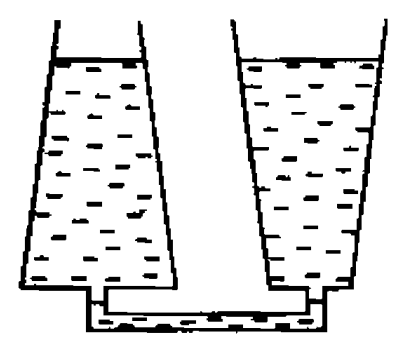
\includegraphics[scale=0.3]{images/19.png}
		\end{center}

\textbf{27.} მაგიდაზე მჭიდროდ დევს ნახევრად სფერული ზარხუფი, რომელშიც უმაღლეს წერტილში გაკეთებული ხვრელიდან ასხამენ წყალს. როცა ზარხუფი აივსება, წყალი ასწევს მას და გამოედინება ქვემოდან. იპოვეთ ზარხუფის მასა $M$, თუ მისი რადიუსია $R$, წყლის სიმკვრივე კი $\rho$.
		\begin{center}
			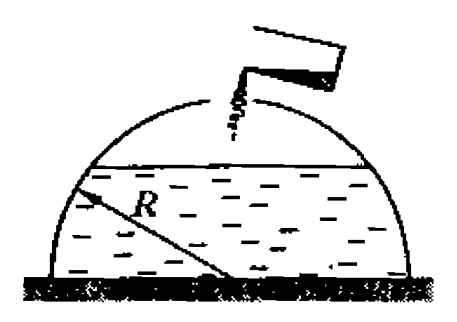
\includegraphics[scale=0.3]{images/27.png}
		\end{center}
	
\textbf{32.} წყლის ზედაპირზე დაცურავს ხის კვადრატული განიკვეთის ნაჭერი. სურათზე გამოსახული ორი მდგომარეობიდან რომელი იქნება მდგრადი. ხის ნაჭრის სიმკვრივე წყლის სიმკვრივის ნახევრის ტოლია.
		\begin{center}
			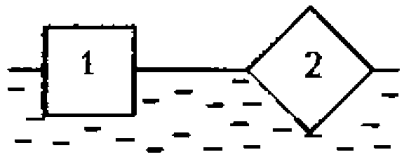
\includegraphics[scale=0.5]{images/32.png}
		\end{center}

\textbf{37.} ორი ვერტიკალურ შეერთებულ ცილინდრული ჭურჭლებში, განიკვეთებით $S_1$ და $S_2$, მოთავსებულია $l$ სიგრძის უმასო ძაფით შეერთებული, ორი უმასო დგუში. დგუშებს შორის მოცულობა შევსებულია წყლით. განსაზღვრე ძაფის დაჭიმულობა, თუკი ჭურჭლების ბოლოები ღიაა ატმოსფეროში. წყლის სიმკვრივეა $\rho$.
		\begin{center}
			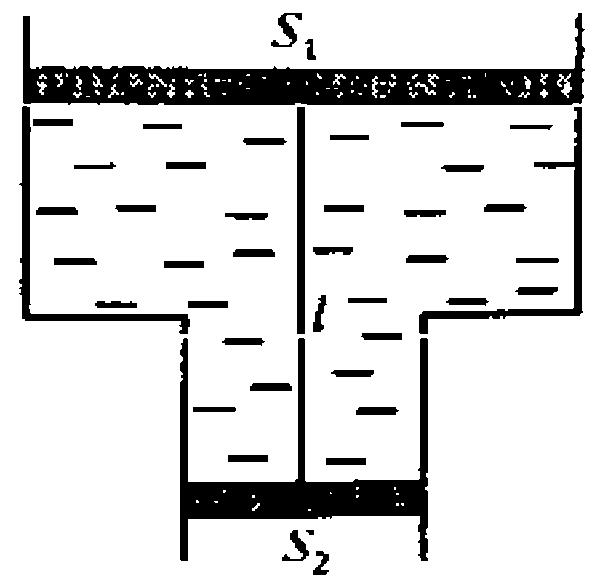
\includegraphics[scale=0.2]{images/F37.jpg}
		\end{center}

\textbf{44.} ორი დელფინი მიცურავს შემხვედრი მიმართულებით. ერთერთი მათგანი გამოსცემს $f$ სიხშირის ბგერებს. რა სიხშირის ხმა ესმის მეორე დელფინს, თუ დელფინების სიჩქარე წყლის მიმართ ერთნაირია და მოდულით $v$-ს ტოლია ? ბგერის სიჩქარე წყალში უდრის $u$.

\textbf{52.} ბურთი ააგდეს ვერტიკალურად ზევით. რომელია მეტი: ზევით მოძრაობის დრო თუ ქვევით მოძრაობის დრო ?

\textbf{54.} რას აჩვენებს ამპერმეტრი სურათზე გამოსახულ სქემაში ? ამპერმეტრის წინაღობა ძალიან მცირეა. 
		\begin{center}
			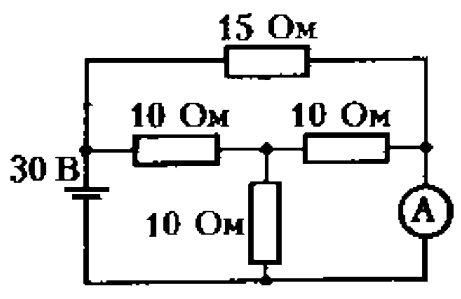
\includegraphics[scale=0.4]{images/54.png}
		\end{center}
	
\textbf{63.} მოყინულ დაღმართზე რომ არ მოცურდეს, ადამიანი ჩამორბენას ამჯობინებს. რატომ ? 
	
\textbf{??.} ნავში წყლის დონე ემთხვევა წყლის დონეს ტბაში. სად იქნება წყლის დონე მეტი, თუ ნავში ჩავაგდებთ ხის ნაფოტს.

\textbf{96.} ორი ერთნაირი ბურთულა შეერთებულია ძაფით. განსაზღვრეთ რა სიმაღლეს მიაღწევს ეს სისტემა, თუკი ერთერთ ბურთულას ავაგდებთ ზევით $v$ სიჩქარით. 

\textbf{144.} როგორი უნდა იყოს ერთგვაროვანი ღეროს იატაკთან ხახუნის კოეფიციენტი, რომ ის გაჩერდეს ისე როგორც სურათზეა ნაჩვენები ? ღეროს სიგრძე უდრის დამჭერი ძაფის სიგრძეს. 
		\begin{center}
			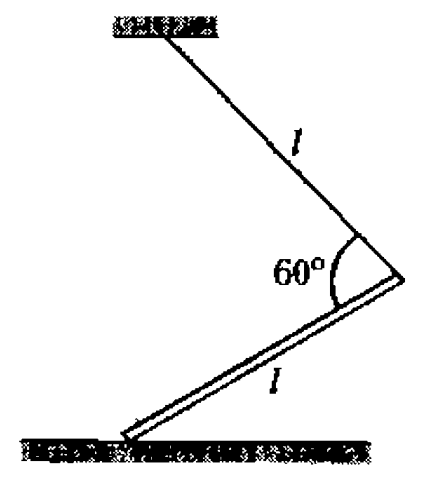
\includegraphics[scale=0.3]{images/144.png}
		\end{center}

\textbf{164.} $M=100$ გ მასის პენოპლასტის კუბი დევს ჰორიზონტალურ სადგამზე. კუბის სიმაღლეა $a=10$ სმ. კუბს ქვემოდან ხვრეტს $m=10$ გ მასის ტყვია, რომლის სიჩქარე კუბში შესვლისას $v_1=100$ მ/წმ, გამოსვლისას $v_2=95$ მ/წმ. მოცილდება თუ არა კუბი სადგამს ? 
		\begin{center}
			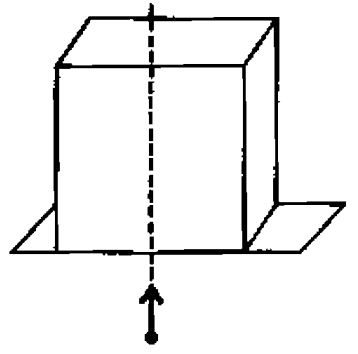
\includegraphics[scale=0.4]{images/164.png}
		\end{center}
	
\textbf{179.} წყალქვეშა ნავი წყალში ვერტიკალურად ჩასვლისას ფსკერის მიმართულებით ასხივებს ხანმოკლე ბგერით ტალღებს ხანგრძლივობით $\tau_0$. ფსკერიდან არეკლილი სიგნალების ხანგრძლივობა კი, რომელსაც ნავში მჯდომი ჰიდროაკუსტიკოსი ზომავს აღმოჩნდა $\tau$. რა სიჩქარით იძირება ნავი ? ბგერის სიჩქარე წყალში ტოლია $v$. ფსკერი ჰორიზონტალურია.

\textbf{188.} $P$ სიმძლავრის მაცივარმა $\tau$ დროში ყინულად გადააქცია $n$ მოცულობის წყალი, რომელსაც საწყისი ტემპერატურა გააჩნდა $t$. განსაზღვრე რა რაოდენობის სითბო გამოიყო ოთახში.
 
\textbf{297.} კონუსის ფორმის საცობი ერთდროულად ორ ნახვრეტს კეტავს ბრტყელ ჭურჭელში, რომელშიც ჩასხმულია სითხე $P$ წნევით.  ნახვრეტების რადიუსია $R$ და $r$. განსაზღვრე საცობზე სითხის მხრიდან მოქმედი ძალა. სიმძიმის ძალა არ გაითვალისწინოთ.
		\begin{center}
			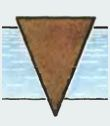
\includegraphics[scale=0.5]{images/F297.jpg}
		\end{center}

\textbf{338.} ორი განსხვავებული ლითონისგან, წრფივი გაფართოების კოეფიციენტებით $\beta_1$ და $\beta_2$, დამზადებულ ღეროს, $0\degree$ ტემპერატურაზე გააჩნიათ მცირედ განსხვავებული $l_1$ და $l_2$ სიგრძეები. რა ტემპერატურაზე იქნება ტოლი მათი: ა) სიგრძეები? ბ) განივი კვეთები გ) მოცულობები?

\textbf{423.} საჰაერო ბურთი მიწაზე მიათრევს გვარლს. საჰაერო ბურთისა და გვარლის მასა ერთად არის $M$. ბურთზე მოქმედი ამომგდები ძალაა $F$, მიწაზე გვარლის ხახუნის კოეფიციენტი - $\mu$. ბურთზე მოქმედი ჰაერის წინააღმდეგობის ძალა ჰაერის მიმართ ბურთის სიჩქარის პროპორციულია $F_r=\alpha v$. იპოვეთ ბურთის სიჩქარე დედამიწის მიმართ, თუ ქრის $u$ სიჩქარის ჰორიზონტალური ქარი.

\textbf{524.} 

\textbf{579.} სურათზე გამოსახულ სქემაში, $R_1=10$ ომი, $R_2=20$ ომი, $R_3=15$ ომი, ქსელში ცვლადი დენის ძაბვაა $U=10$ ვოლტი. განსაზღვრეთ რა სიმძლავრე გამოიყოფა $R_2$ და $R_3$ წინაღობებზე. 
		\begin{center}
			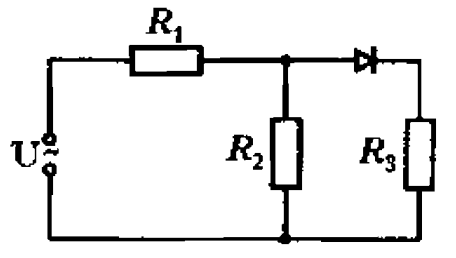
\includegraphics[scale=0.5]{images/F579.png}
		\end{center}
	
\textbf{649.} ვედროში ასხია წყლის და ყინულის ნარევი. ნარევის მასაა 10 კგ. ვედრო შეიტანეს ოთახში და მაშინვე დაიწყეს ნარევის ტემპერატურის გაზომვა. მიღებული ტემპერატურის დროზე $t(\tau)$ დამოკიდებულება მოყვანილია გრაფიკზე. წყლის კუთრი სითბოტევადობა $c=4.2\cdot10^3$ ჯ/(კგ$\cdot K$), ყინულის დნობის კუთრი სითბო $\lambda=3.4\cdot10^5$ ჯ/კგ. განსაზღვრეთ რა მასის ყინული იყო ვედროში თავდაპირველად. ვედროს სითბოტევადობა უგულებელყავით. 
		\begin{center}
			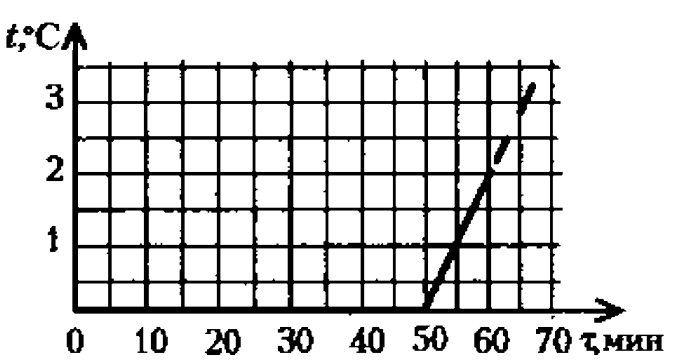
\includegraphics[scale=0.5]{images/F649.png}
		\end{center}

\textbf{683.} სურათზე გამოსახულია $AB$ წყარო და მისი ლინზაში მიღებული $A'B'$ გამოსახულება. აგებით განსაზღვრეთ ლინზის მდებარეობა და მისი ფოკუსური მანძილი. 
		\begin{center}
			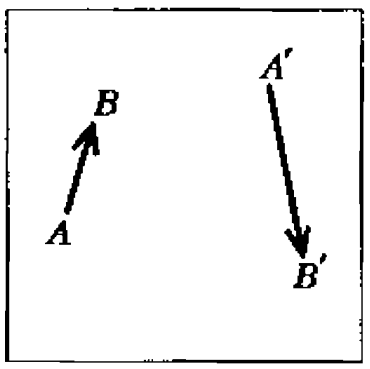
\includegraphics[scale=0.5]{images/F683.png}
		\end{center}
	
\textbf{723.} $l_0$ სიგრძის სპორტსმენების კოლონა მირბის $v$ სიჩქარით. მათ შესახვედრად მორბის მწვრთნელი $u<v$ სიჩქარით. ყოველი სპორსტმენი შეხვდება რა მწვრთნელს, ბრუნდება და უკან გარბის მოდულით იგივე $v$ სიჩქარით. რა სიგრძის გახდება კოლონა მას შემდეგ როცა ყველა სპორტსმენი შემობრუნდება.
		
\textbf{724.} რამდენით ჩამოიწევს თოკის $A$ ბოლო, რომელიც გადაკიდებულია მოძრავ ჭოჭონაქზე, თუ მას მოვდებთ $F$ ძალას ? ზამბარების სიხისტეა $k$. ზამბარა, თოკი და ჭოჭონაქი უმასოა.
		\begin{center}
			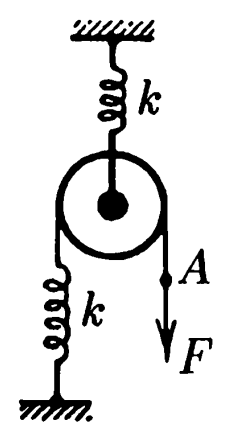
\includegraphics[scale=0.3]{images/724.png}
		\end{center}

\textbf{754.} ჭიანჭველა მოძრაობს წრფივად და ბუდეს სცილდება სიჩქარით, რომელიც ბუდის ცენტრიდან მანძილის უკუპროპორციულად იცვლება. იმ მომენტში, როცა ჭიანჭველა იმყოფება $A$ წერტილში, ბუდის ცენტრიდან იგი დაშორებულია $l_1=1$ მ-ით და მისი სიჩქარე ტოლია  $v_1=2$ მ/წმ. რა $t$ დროში მიაღწევს ჭიანჭველა $A$ წერტილიდან $B$ წერტილში, რომელიც ბუდის ცენტრიდან დაშორებულია $l_2=2$ მ მანძილით ? 

\textbf{761.} 

\textbf{783.} 

\textbf{844.} ჭურჭელში რომელშიც ჩასხმული სითხის სიმკვრივე სიღრმის მიხედვით იცვლება კანონით $\rho=\rho_0+\alpha h$, ჩაუშვეს $m$ მასისა და $V$ მოცულობის სხეული. სხეული სრულად იძირება სითხეში. რა სიღრმეზე გაჩერდება სხეული თუ ის კუბური ფორმისაა? სფეროს ფორმისაა?

\textbf{1006.} განსაზღვრეთ სურათზე გამოსახული წრედის საერთო წინაღობა. ცალკეული წინაღობების მნიშვნელობები მითითებულია ომებში. 
		\begin{center}
			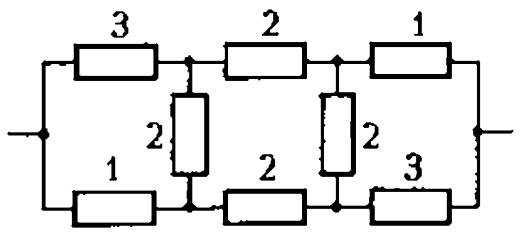
\includegraphics[scale=0.4]{images/1006.png}
		\end{center}

\textbf{1015.} სურათზე მოცემული სქემა შედგება 50 განსხვავებული ამპერმეტრისა და 50 ერთნაირი ვოლტმეტრისაგან. პირველი ვოლტმეტრი აჩვენებს $U_1=9.6$ ვ, პირველი ამპერმეტრი $I_1=9.5$ მა, მეორე ამპერმეტრი $I_1=9.5$ მა-ს. ამ მონაცემებით გამოთვალეთ ყველა ვოლტმეტრების ჩვენებათა ჯამი. 
		\begin{center}
			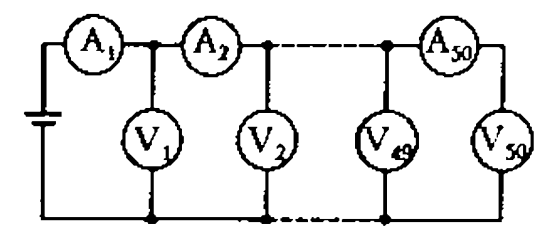
\includegraphics[scale=0.4]{images/1015.png}
		\end{center}

\textbf{1065.} ქვაბში ჩასხმული 1 ლ წყალი 100 ვტ სიმძლავრის სახურებლით ვერა და ვერ აადუღეს. რამდენ ხანში შემცირდება წყლის ტემპერატურა 1 გრადუსით, თუ სახურებელს გამოვრთავთ ?

\textbf{1071.} სურათზე გამოსახულ სქემაზე ნათურა ერთნაირად ანათებს იმის მიუხედავად, ჩაკეტილია თუ ღიაა $K$ ჩამრთველი. ძაბვა დენის წყაროს მომჭერებზე $U=54$ ვ, $R_1=R_3=90$ ომი, $R_2=180$ ომი. იპოვეთ ძაბვა ნათურის ბოლოებზე.
		\begin{center}
			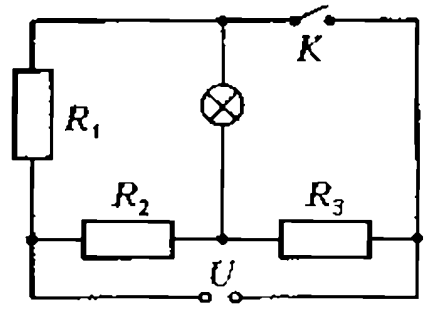
\includegraphics[scale=0.3]{images/F1071.png}
		\end{center}
	
\textbf{1124.} ჰორიზონტალურად დადებულ მორზე, რომლის რადიუსია $R$, ჩამოდებულია „წიგნი“, შედგენილი კვადრატული ფირფიტისაგან, ფირფიტის გვერდის სიგრძეა $l=4R$. ფირფიტები ერთმანეთთან შეერთებულია უმასო სახსარით. როგორი კუთხე იქნება ფირფიტებს შორის წონასწორობის დროს ? იქნება თუ არა ეს წონასწორობა მდგრადი ?
		\begin{center}
			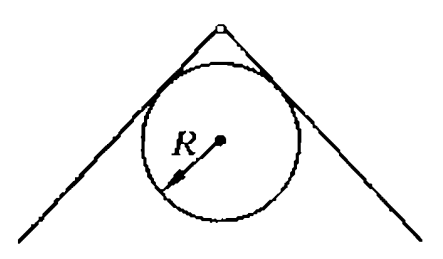
\includegraphics[scale=0.2]{images/F1124.png}
		\end{center}

\textbf{1215.} 1 კგ ყინული და 1 კგ ადვილად დნობადი ნივთიერება, რომელიც არ ერევა წყალს, $-40\ \degree C$-ზე მოათავსეს თბოიზოლირებულ ჭურჭელში, გამაცხელებლით შიგნით. გამათბობელის სიმძლავრე მუდმივია. ჭურჭელში ტემპერატურის დროზე დამოკიდებულების გრაფიკი მოცემულია. ყინულის კუთრი სითბოტევადობა $2.1\cdot10^3$ ჯ/(კგ$\cdot K$), ადვილად დნობადი ნივთიერების მყარ მდგომარეობაში $10^3$ ჯ/(კგ$\cdot K$). განსაზღვრე ადვილად დნობადი ნივთიერების დნობის კუთრი სითბო და მისი კუთრი სითბოტევადობა თხევად მდგომარეობაში.
		\begin{center}
			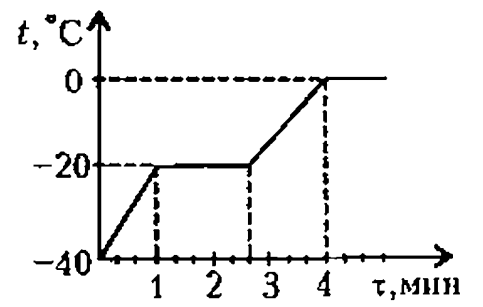
\includegraphics[scale=0.5]{images/F1215.png}
		\end{center}
	
\textbf{1258.} ჰორიზონტალურ მაგიდაზე მოთავსებულია $R$ რადიუსიანი კოჭა. მასზე დახვეულია წვრილი უწონო ძაფი. ნახვევის რადიუსია $r$. ძაფი გატარებულია მცირე ხვრელში, რომელიც მაგიდის ზედაპირიდან $h$ სიმაღლეზეა $(h>R)$. საწყის მომენტში კოჭა უძრავია, ხოლო ძაფი ვერტიკალურია. რაღაც მომენტში დაიწყეს ძაფის გაწევა მუდმივი $F$ ძალით და კოჭა გაგორდა მაგიდაზე სრიალის გარეშე. განსაზღვრე კოჭას მაქსიმალური სიჩქარე. კოჭას მასაა $M$. ჩათვალე, რომ კოჭის მასის ნახევარი მისი ღერძის მასაა, ხოლო მეორე ნახევარი თანაბრადაა განაწილებული $R$ რადიუსის ფერსოზე. ძაფი გლუვად მიიჩნიე.
		\begin{center}
			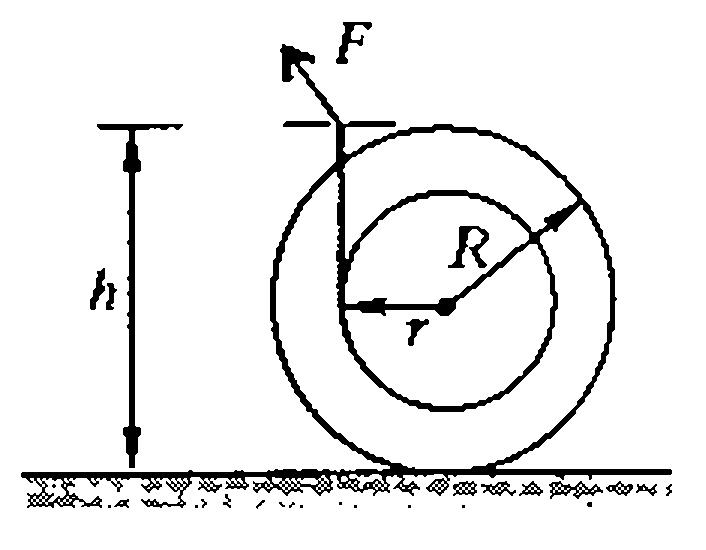
\includegraphics[scale=0.2]{images/F1258.jpg}
		\end{center}

\textbf{1283.} დაშვებულ შლაგბაუმთან დგას ადამიანი დატვირთული ურიკით. მან უმცირეს დროში უნდა მიიტანოს ტვირთი მაღაზიაში, რომელიც შლაგბაუმიდან 300 მეტრითაა დაშორებული. მაქსიმალური ძალა რომლითაც ადამიანს შეუძლია იმოქმედოს ურიკაზე 500 ნ-ია, დატვირთული ურიკის მასაა 2000 კგ, ხოლო მაქსიმალური სიჩქარე რომლითაც ურიკის მოძრაობა შეიძლება $v=5$ მ/წმ. ცნობილია რომ შლაგბაუმი გაიხსნება ზუსტად $t_0=30$ წამის შემდეგ. რა მინიმალურ $\tau$ დროში მიიტანს ადამიანი ტვირთს მაღაზიაში ? 

\textbf{1292.} წერტილოვანი სინათლის წყაროდან 20 სმ-ში მოთავსებულია 1 სმ დიამეტრისა და 10 სმ ფოკუსური მანძილის მქონე შემკრები ლინზა. ამავე წყაროდან 50 სმ-ში მოთავსებულია 10 სმ დიამეტრისა და 20 სმ ფოკუსური მანძილის მქონე მეორე შემკრები ლინზა. ლინზებს საერთო მთავარი ოპტიკური ღერძი აქვთ და სინათლის წყარო ამ ღერძზეა განლაგებული. დიდი ლინზის შემდეგ რა მანძილზე უნდა მოვათავსოთ ეკრანი იმისათვის, რომ სინათლის ლაქას ამ ეკრანზე ქონდეს მინიმალური ზომა? იპოვეთ ამ ლაქის დიამეტრი. როგორ შეიცვლება ლაქის განათებულობა, პატარა ლინზას თუ მოვაშორებთ ?

\textbf{1320.} სურათზე გამოსახულ სქემაზე, ბატარეა იდეალურია, რეზისტორები გარდა $R_x$ და $R_y$-სა გააჩნიათ ერთნაირი $10$ ომი წინაღობა. $A$ და $B$ წერტილებს შორის ძაბვაა $10$ ვ, ხოლო $B$ და $C$ წერტილებს შორის - $2$ ვ. იპოვეთ $R_x$ და $R_y$ წინაღობების მნიშვნელობები.
		\begin{center}
			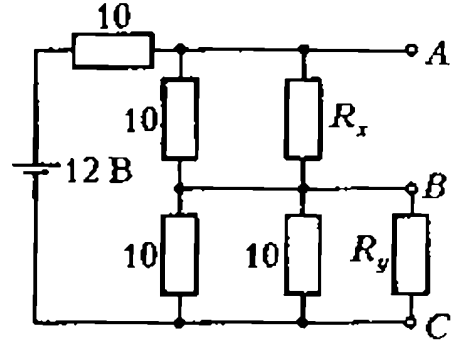
\includegraphics[scale=0.4]{images/F1320.png}
		\end{center}
	
\textbf{1328.} $M$ მასის სოლი, რომლის დახრილი წახნაგის სიგრძეა $L$ და ფუძესთან კუთხეა $\alpha$, მოთავსებულია გლუვ ჰორიზონტალურ ზედაპირზე (იხილე ნახაზი). სოლის ზედა წერტილთან მიმაგრებულია ძალიან თხელი ლენტის ერთი ბოლო. ლენტის მასაა $m=M/3$, ხოლო სიგრძეა $L$. ლენტი ბოლომდე დაახვიეს გორგლად და ამის შემდეგ სისტემა გაანთავისუფლეს. განსაზღვრეთ სოლის მაქსიმალური სიჩქარე. ხახუნი უგულებელყავით.                                                                   
		\begin{center}
			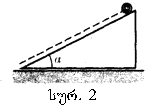
\includegraphics[scale=0.5]{images/F1328.png}
		\end{center}

\textbf{1332.} თხელ ლინზაზე დაცემული სხივი მის მთავარ ოპტიკურ ღერძს კვეთს $\alpha = 4 \degree$ კუთხით ლინზიდან $d=12$ სმ მანძილზე და გარდატეხის შემდეგ გამოდის $\beta = 8 \degree$ კუთხით მთავარ ოპტიკურ ღერძთან. იპოვეთ ლინზის მთავარი ფოკუსური მანძილი.

\textbf{1347.} შუშიდან დამზადებულს თხელ სფერულ ლინზას აქვს $d=3$ მმ სისქე და $D=4$ სმ დიამეტრი. ეს ლინზა ბრტყლად დადეს წყლის ზედაპირზე ისე, რომ იგი ნახევრად ჩაძირულია წყალში. ამ დროს ზენიტში მყოფი მზის გამოსახულება აღმოჩნდა წყალში $h_1=17,5$ სმ სიღრმეზე. როდესაც ლინზა ამოაბრუნეს და  მეორე მხრიდან ჩაძირეს ნახევრად წყალში, მაშინ მზის გამოსახულება აღმოჩნდა $h_2=13,5$ სმ სიღრმეზე. რისი ტოლია ლინზის ზედაპირების სამრუდის რადიუსები? წყლის გარდატეხის მაჩვენებელია $n=1,33$.

\textbf{1387.} $N$ შემკრები ლინზა, რომელთა ფოკუსური მანძილებია $2F$ და $N$ გამბნევი ლინზა, რომელთა ფოკუსური მანძილებია $F$. ეს ლინზები განლაგებულია საერთი ღერძის გასწვრივ ერთმანეთისაგან $F$ მანძილზე ისე, როგორც ნახატზეა ნაჩვენები. ამ ღერძის გასწვრივ ლინზათა სისტემას ეცემა $D$ დიამეტრის მქონე პარალელურ სხივთა კონა. რისი ტოლია სისტემიდან გამოსული კონის დიამეტრი? გასასწორებელია. 
		
\textbf{1388.} გლუვი მავთული მოღუნულია ჰორიზონტალურ სიბრტყეში ისე, რომ აქვს $y=\alpha x^2$ პარაბოლის ფორმა. მავთულის გასწვრივ მოდულით $v_0$ მუდმივი   სიჩქარით მისრიალებს $m$ მასის მძივის მარცვალი. იპოვე რა ძალით აწვება მარცვალი მავთულს პარაბოლის წვეროს გავლისას.                            
		\begin{center}
			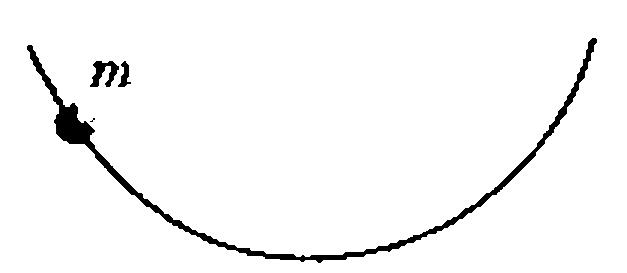
\includegraphics[scale=0.2]{images/F1388.jpg}
		\end{center}

\textbf{1389.} $L$ სიგრძის უწონო $OA$ ღეროს, რომლის ბოლოში მიმაგრებულია $m$ მასის ტვირთი,  შეუძლია ხახუნის გარეშე ბრუნვა მაგიდის ზედაპირის $O$ წერტილის გარშემო (იხილე ნახაზი). $M$ მასის მეორე ტვირთი მიმაგრებულია პირველ ტვირთთან უჭიმვადი ძაფით, რომელიც გატარებულია $O$ წერტილიდან $L/2$ დაშორებით მაგიდაში არსებულ მცირე ხვრელში. საწყის მომენტში ღერო მოყავთ ვერტიკალურ მდებარეობაში და ათავისუფლებენ საწყისი სიჩქარის მინიჭების გარეშე. განსაზღვრეთ $m$ მასის ტვირთის სიჩქარე უშუალოდ მაგიდასთან დაჯახების წინ.
		\begin{center}
			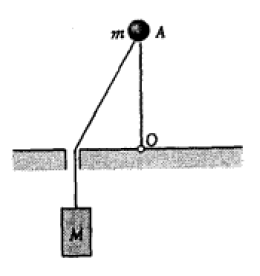
\includegraphics[scale=0.4]{images/F1389.png}
		\end{center}
	
\textbf{1418.} $R$ რადიუსის წრეწირზე მუდმივი სიჩქარით დარბის ცხენი. წრეწირის ცენტრიდან $r$ მანძილზე დგას ადამიანი. რისი ტოლია ადამიანისა და ცხენის მაქსიმალური დაახლოების სიჩქარე ? 

\textbf{1488.} ოთახის კუთხეში ვერტიკალურად დგას ჰანტელი, რომელიც შედგება $l=0.1$ მ სიგრძის  მსუბუქი ღეროთი შეერთებული ორი ერთნაირი მასიური ბურთულასაგან (იხილე ნახაზი). ზედა ბურთულას ბიძგით მიანიჭეს კედლიდან მიმართული $v_0=1$ მ/წმ ჰორიზონტალური სიჩქარე, ქვედა ბურთულა ამ მომენტში უძრავია. განსაზღვრეთ ზედა ბურთულას სიჩქარე იატაკზე დაჯახების მომენტში.
		\begin{center}
			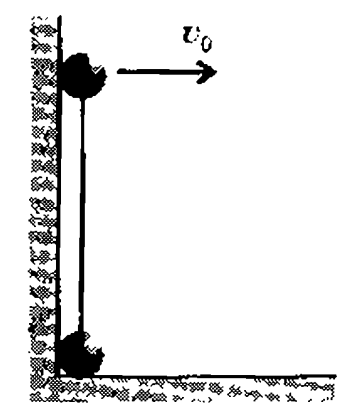
\includegraphics[scale=0.4]{images/F1488.png}
		\end{center}
	
\textbf{1489.} გლუვ დამაგრებულ დახრილ სიბრტყეზე აკავებენ $M$ მასის სოლს (იხილე ნახაზი). სოლის ზედა წახნაგი ჰორიზონტალურია. მასზე მოთავსებულია $5M$ მასის კუბიკი. სოლს ათავისუფლებენ და ის იწყებს სრიალს დახრილ სიბრტყეზე. რისი ტოლი შეიძლება იყოს მისი მაქსიმალური აჩქარება?
		\begin{center}
			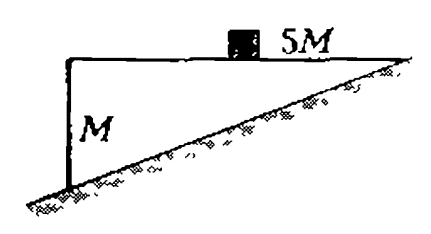
\includegraphics[scale=0.4]{images/F1489.png}
		\end{center}

\textbf{1490.} მაგიდის ჰორიზონტალურ ზედაპირზე მოთავსებულია გორაკის ფორმის გლუვი სხეული, რომელსაც შეუძლია მაგიდაზე ხახუნის გარეშე სრიალი. მისი სიმაღლეა $H$ და ფუძის სიგრძეა $L$. გორაკისკენ მიგორავს პატარა ურიკა, რომლის მასა 3-ჯერ ნაკლებია გორაკის მასაზე. ურიკის სიჩქარეა $v$. იპოვეთ, რამდენით წაინაცვლებს გორაკი  იმ მომენტისათვის, როდესაც ურიკა დატოვებს მას. ურიკას გორაკზე მოძრაობის დროა $T$. 
		\begin{center}
			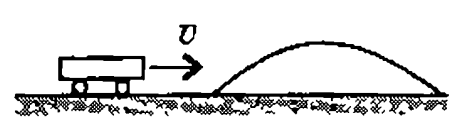
\includegraphics[scale=0.4]{images/F1490.png}
		\end{center}
	
\textbf{1508.} რკინის $R$ რადიუსის ღეროზე წამოცმულია რეზინის რგოლი. რგოლის დაჭიმულობის ძალაა $T$. რა ძალა უნდა მოვდოთ რგოლს რომ იგი გავაჩოჩოთ ღეროს გასწვრივ ? ძალა თანაბრადაა განაწილებული რგოლზე. ხახუნის კოეფიციენტი რეზინა-რკინის საზღვარზე ტოლია $\mu$. 

\textbf{1587.} გრძელ ჰორიზონტალურ გლუვ ცარიელ მილში იმყოფება ორი დგუში, რომლებსაც ხახუნის გარეშე შეუძლიათ სრიალი მილის გასწვრივ. ერთი დგუშის მასაა $M=1$ კგ, ხოლო მეორის - ორჯერ მეტი. საწყის მომენტში დგუშებს შორის იმყოფება $T_0=300~K$ ტემპერატურის ერთი მოლი ჟანგბადი, ხოლო მძიმე დგუში $v_0=1$ მ/წმ სიჩქარით მოძრაობს ამ მომენტში უძრავი მსუბუქი დგუშისკენ. რისი ტოლია აირის მაქსიმალური ტემპერატურა შემდგომ პროცესში? განსაზღვრეთ დგუშების სიჩქარეები დიდი დროის შემდეგ. მილის და დგუშების სითბოტევადობა მცირეა, თბოგამტარობა უგულებელყავით.

\textbf{1589.} რეზისტორების გრძელი ჯაჭვი შეიცავს მორიგეობით ჩართულ $2R-R$ და $R-2R$ ტიპის რგოლებს, როგორც ნაჩვენებია ნახ. ზე. განსაზღვრეთ წინაღობა $A$ და $B$ წერტილებს შორის რგოლების დიდი რიცხვის შემთხვევაში.  
		\begin{center}
			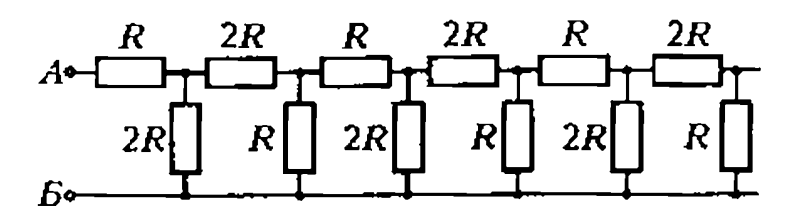
\includegraphics[scale=0.4]{images/F1589.png}
		\end{center}

\textbf{1599.} ორი, თითოეული $L$ სიგრძის ღერო სახსრულადაა შეერთებული. ერთი ღეროს თავისუფალი ბოლო სახსრულადაა დამაგრებული, ხოლო მეორე ღეროს თავისუფალი ბოლო თანაბრად და წრფივად იწყებს მოძრაობას $\vec{v_0}$ სიჩქარით. საწყის მომენტში სიჩქარის ვექტორი ღეროებს შორის $2\alpha$ კუთხის ბისექტრისის პარალელურია. განსაზღვრეთ ღეროების შემაერთებელი სახსრის აჩქარების მოდული და მიმართულება საწყის მომენტში. 
		\begin{center}
			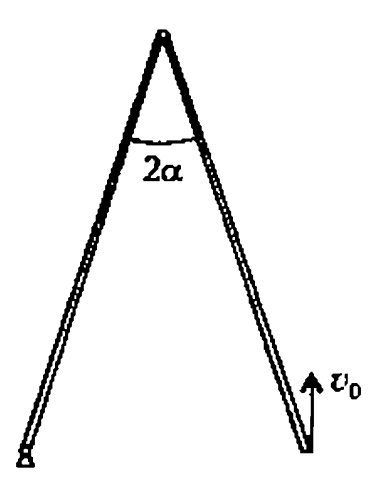
\includegraphics[scale=0.4]{images/F1599.png}
		\end{center}
	
\textbf{1601.} $R$ რადიუსიან ხისტ უწონო რგოლზე მიმაგრებულია მცირე ზომის სხეული. რგოლს აკავებენ სურათზე გამოსახულ მდებარეობაში. ვერტიკალური კედლიდან რა მანძილზე შეეხება სხეული ჰორიზონტალურ სიბრტყეს რგოლის განთავისუფლების შემდეგ? ხახუნი უგულებელყავით.               
		\begin{center}
			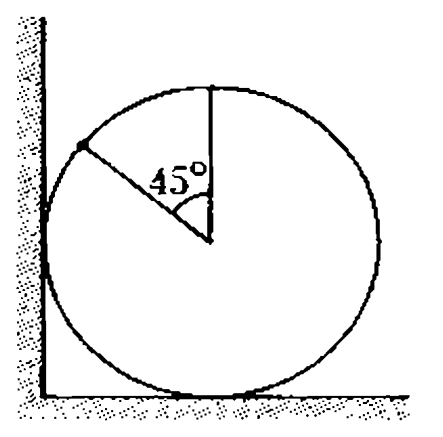
\includegraphics[scale=0.4]{images/F1601.png}
		\end{center}
	
\textbf{1609.} მქისე ჰოროზონტალურ ზედაპირზე დევს ორი ერთნაირი გრძელი თხელკედლიანი მილი. მათი ღერძები პარალელურია. ერთი მილი უძრავია, მეორე კი მისკენ მიგორავს სრიალის გარეშე სიჩქარით. ხდება აბსოლუტურად დრეკადი დაჯახება (დაჯახებისას მილებს შორის ხახუნი შეიძლება უგულებელვყოთ). ზედაპირსა და მილებს შორის სრიალის ხახუნის კოეფიციენტია $\mu$. განსაზღვრეთ მილებს შორის მაქსიმალური მანძილი დაჯახების შემდეგ.

\textbf{1610.} ჰელიუმის  დაყვანილი ტემპერატურის $T/T_0$ დამოკიდებულება $p/p_0$ დაყვანილ წნევაზე გამოისახება წრეწირით, რომლის ცენტრი $(1; 1)$ წერტილშია. ამასთან, ამ პროცესში ჰელიუმის მინიმალური დაყვანილი ტემპერატურაა $\tau_m$ . განსაზღვრეთ ამ პროცესში ჰელიუმის ატომების მინიმალური და მაქსიმალური კონცენტრაციათა შეფარდება.

\textbf{1613.} გლუვ ჰორიზონტალურ მაგიდაზე მოთავსებულია $M$ მასის ურიკა. მასზე მოთავსებულია ჭოჭონაქზე გადადებული წვრილი, მსუბუქი ძაფით შეერთებული $5M$ და $M$ მასების ორი კუბიკი. ჭოჭონაქს ქაჩავენ ჰორიზონტალურად მიმართული მუდმივი ძალით. ძაფის ნაწილები ამ დროს ჰორიზონტალურია. კუბიკებსა და ურიკის ზედაპირს შორის ხახუნის კოეფიციენტია $\mu=0.1$. განსაზღვრეთ გამწევი ძალის მოდულის რა მნიშვნელობისათვის იქნება ურიკის აჩქარება $a=0.2g$ . რისი ტოლია ამ დროს კუბიკების და ჭოჭონაქის აჩქარებები?                         
		\begin{center}
			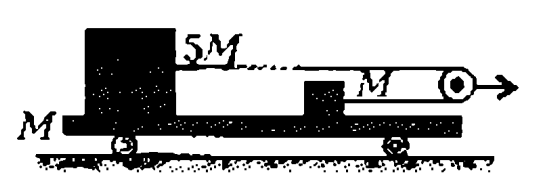
\includegraphics[scale=0.4]{images/F1613.png}
		\end{center}

\textbf{1614.} გლუვ ჰორიზონტალურ მაგიდაზე იმყოფება $M$ მასის ურიკა. მასზე ვერტიკალურად დგას $3M$ მასის ველოსიპედის ბორბალი. ურიკასა და ბორბალს შორის ხახუნის კოეფიციენტია $\mu$. ურიკას მოსდეს ბორბლის ზედაპირის პარალელური ჰორიზონტალური მუდმივი ძალა. განსაზღვრეთ ამ ძალის მაქსიმალური მნიშვნელობა, რომლის დროსაც ბორბალი ჯერ კიდევ მოძრაობს ურიკაზე გასრიალების გარეშე. ჩათვალეთ, რომ ბორბლის მასა თანაბრადაა განაწილებული მის ფერსოზე - გარე წრეწირზე.         
		\begin{center}
			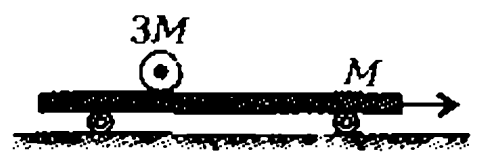
\includegraphics[scale=0.4]{images/F1614.png}
		\end{center}

\textbf{1617.} ვერტიკალურ თბოიზოლირებულ ჭურჭელში მასიური მოძრავი დგუშის ქვეშ იმყოფება $T_0$ ტემპერატურის იდეალური ერთატომიანი აირის პორცია. დგუში ამ დროს წონასწორობაშია. ჭურჭელში აირის ტემპერატურა ორჯერ გაზარდეს  მინიატურული სახურებლით ძალიან სწრაფად და სისტემა თავის ნებაზე დატოვეს. განსაზღვრეთ რა ტემპერატურა დამყარდება ჭურჭელში მას შემდეგ, რაც შეწყდება დგუშის მოძრაობა. კედლებთან დგუშის ხახუნი ძალიან მცირეა. დგუში და ჭურჭელი პრაქტიკულად არ იღებს სითბოს აირიდან. გარეთ არ არის ჰაერი.

\textbf{1618.} ხის თბოგამტარობა ბოჭკოების გასწვრივ 2-ჯერ მეტია, ვიდრე მათ მართობულად. ასეთი ხისგან დაამზადეს ერთნაირი ზომების ორი გრძელი და თხელი ცილინდრი. ერთი მათგანის ღერძი ბოჭკოების გასწვრივია, მეორესი კი ბოჭკოების მიმართულებასთან $30 \degree$ კუთხეს ქმნის. გააკეთეს ცილინდრების გვერდითი ზედაპირების თბოიზოლაცია და ფუძეებს შორის შექმნეს ერთნაირი ტემპერატურათა სხვაობა. განსაზღვრეთ, რამდენჯერ განსხვავდება სითბური ნაკადები ამ ცილინდრებში.

\textbf{1624.} საწყის მომენტში ორ პატარა, ერთნაირი - $M$ მასის ბურთულას შორის მანძილია $L$. ამ მომენტში მათ აქვთ ცენტრების შემაერთებელი მონაკვეთის მართობული და ურთიერთსაწინააღმდეგოდ მიმართული მოდულით $v_0$ სიჩქარეები. გარე ძალები არ გვაქვს. გაითვალისწინეთ მხოლოდ ბურთულების გრავიტაციული მიზიდვა. იპოვეთ ბურთულებს შორის მაქსიმალური მანძილი და მათი მინიმალური სიჩქარეები შემდგომი მოძრაობისას. 

\textbf{1625.} $V=1\ \text{მ}^3$ მოცულობის კუბის ფორმის ჭურჭელში იმყოფება $T=300$ K ტემპერატურისა და $p=10^5$ პა წნევის ჰელიუმი. ჭურჭლის კედელში გახსნეს $S=1\ \text{სმ}^2$ ფართობის ხვრელი და $\tau=0.01$ წმ-ს შემდეგ დახურეს. გარეთ ვაკუუმია. შეაფასეთ აირის ტემპერატურის ცვლილება ჭურჭელში სითბური წონასწორობის დამყარების შემდეგ. ჩათვალეთ, რომ ხვრელის გახსნას და დაკეტვას ძალზე ფრთხილად ახდენენ - აირის ზედმეტი ნაკადის შეუქმნელად.

\textbf{1628.} 20 სმ რადიუსიანი წრიული ფირფიტა თანაბრად ბრუნავს ჰორიზონტალურ სიბრტყეში ცენტრში გამავალი ფირფიტის მართობული ღერძის გარშემო. მისი ბრუნვის სიხშირეა 33 ბრ/წთ. ფირფიტის ცენტრიდან კიდისაკენ რადიუსის გასწვრივ მიცოცავს პატარა ზომის ხოჭო. ფირფიტის მიმართ ხოჭოს სიჩქარის მოდული 10 სმ/წმ-ია.ხოჭოსა და ფირფიტას შორის რა მინიმალური ხახუნის კოეფიციენტის შემთხვევაში მოახერხებს ის ფირფიტის კიდემდე მიცოცებას ?

\textbf{1629.} გლუვ ჰორიზონტალურ ზედაპირზე დგას ორი ერთნაირი კუბიკი. ისინი თითქმის ეხებიან ერთმანეთს წახნაგებით. თითოეული მათგანის მასაა $M$. კუბიკებს ზემოდან ფრთხილად დაადგეს $m$ მასის ერთგვაროვანი ბურთულა, რომელმაც დაიწყო კუბიკების გვერდით გაწევა და ვერტიკალურად ქვევით მოძრაობა. იპოვეთ ბურთულას სიჩქარე უშუალოდ ჰორიზონტალურ სიბრტყესთან დაჯახების წინ. ბურთულის საწყისი სიჩქარე უმნიშვნელოდ მცირეა. ბურთულას რადიუსია $R$, წიბოს სიგრძეა $H$. ხახუნი არსად არ არის.  

\textbf{1630.} გლუვ ჰორიზონტალურ მაგიდაზე მოთავსებულია $M$ მასის და $L$ სიგრძის ურიკა. მის შუაში იმყოფება $m$ მასის მცირე ზომის კუბიკი. კუბიკს ბიძგით მიანიჭეს ურიკის ერთ-ერთი ბორტისკენ მიმართული $v$ სიჩქარე. იპოვეთ ურიკის წანაცვლება იმ მომენტისათვის, როდესაც კუბიკი ისევ ურიკის ცენტრში აღმოჩნდება ბორტებთან 17 დაჯახების შემდეგ. ბორტებთან ბურთულას დაჯახებები აბსოლუტურად დრეკადად ჩათვალეთ.

\textbf{1633.} სითბური მანქანის ციკლი ორი ადიაბატისა და ორი იზოქორისგან შედგება. ერთ-ერთი ადიაბატის საწყისი და საბოლოო ტემპერატურებია შესაბამისად $T_1$ და $T_2$. მუშა სხეული იდეალური აირია. იპოვეთ ამ ციკლის მქკ.   

\textbf{1634.} ფიზიკოსის განკარგულებაშია ორი სითბური რეზერვუარი - ძალიან ცხელი ტემპერატურით $+200\ \degree$C და უბრალოდ ცხელი ტემპერატურით $+70\ \degree$C. გარემოს აქვს მუდმივი $+20\ \degree$C ტემპერატურა. ფიზიკოსს დაავალეს გადასცეს ძალიან ცხელ სხეულს 1000 ჯ სითბოს რაოდენობა, ხოლო უბრალოდ ცხელს 2000 ჯ. რა უმცირესი მექანიკური მუშაობის შესრულებს მოუწევს მას ამისთვის? ცხელი და ძალიან ცხელი სხეულების სითბიტევადობები ძალიან დიდია.

\textbf{1638.} პატარა დრეკადი ბურთულა დახტის ჰორიზონონტალურ ფირფიტაზე ვერტიკალური მიმართულებით. ამასთან ახტომის სიმაღლეა $H$ ფირფიტის მიმართ. ფირფიტა ძალიან ნელა გადაადგილეს  $h$-ით თავისი თავის პარალელურად ქვევით და გააჩერეს. განსაზღვრეთ ახტომის ახალი სიმაღლე ფირფიტის მიმართ. 

\textbf{1639.} ჰორიზონტალურად მოთავსებული ცილინდრული ჭურჭელი მასიური დგუშით ვაკუუმში იმყოფება (იხილე სურათი). $k$ სიხისტის ზამბარა ერთი მხრიდან დამაგრებულია, მეორე მხრიდან კი დგუშს ებჯინება. საწყის მომენტში დგუშში არ არის აირი, ზამბარა არაა დეფორმირებული. ჭურჭლის ფსკერში არსებული ხვრელიდან მასში შეუშვეს ჰელიუმის გარკვეული რაოდენობა და ხვრელი დახურეს. წონასწორობის დამყარების შემდეგ ზამბარა დეფორმირებული აღმოჩნდა $L$-ით. ამის შემდეგ აირს ძალიან ნელა ათბობენ მანამ, სანამ დგუში კიდევ $L$-ით გადაადგილდება. განსაზღვრეთ რა სითბოს რაოდენობა მიიღო აირმა. ჭურჭლის და დგუშის სითბოტევადობა უგულებელსაყოფად მცირეა.
		\begin{center}
			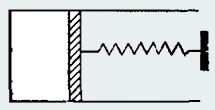
\includegraphics[scale=0.5]{images/F1639}
		\end{center}

\textbf{1647.} კოსმოსში, ყველა სხვა სხეულისაგან დიდ მანძილზე, მოძრაობს ერთი მხრიდან დახშული გრძელი ცილინდრული მილი. მილში არის $M=1$ კგ მასის მიწებებული დგუში, რომელიც ვაკუუმისგან გამოყოფს მილის სრული მოცულობის 1/100 ნაწილს. მილის ამ ნაწილში იმყოფება $T=300$ K ტემპერატურის და $p=0.5$ ატმ წნევის აზოტის მცირე პორცია. გარკვეულ მომენტში დგუში განთავისუფლდა და წნევის მოქმედებით დაიწყო სრიალი მილის გასწვრივ ხახუნის გარეშე. განსაზღვრეთ, მოძრაობის დაწყებიდან რა დროის შემდეგ გამოფრინდება დგუში მილიდან. მილის სიგრძეა $L=5$ მ, ფუძის შიგა ფართობია $A=100\ \text{სმ}^2$ , მილის მასა დგუშის მასაზე 10-ჯერ მეტია.

\textbf{1648.} $V=100$ ლ ტევადობის ჭურჭელში იმყოფება ჰაერი ნორმალურ პირობებში. გარეთ - ვაკუუმია. ჭურჭლის კედელში $\tau=1$ წმ-ის განმავლობაში იღება $S=0.1\ \text{სმ}^2$ ფართობის მცირე ხვრელი და შემდეგ სწრაფად იკეტება. შეაფასეთ ამ დროის განმავლობაში ჭურჭლიდან გამოსული მოლეკულების რიცხვი და მათი ჯამური ენერგია. შევნიშნოთ, რომ ჰაერი - ორატომიანი აირების ნარევია.

\textbf{1653.} აივნიდან დროის ტოლი შუალედების შემდეგ აგდებენ კენჭებს უსაწყისო სიჩქარით. იმ მომენტში, როდესაც პირველი კენჭი დაეცა მიწაზე, მომდევნოს გავლილი ჰქონდა გასავლელი გზის ნახევარი. გზის რა ნაწილი ჰქონდა გავლილი ამ მომენტისათვის მესამე კენჭს? რამდენი კენჭი იყო მოძრაობაში პირველი კენჭის მიწასთან დაჯახების მომენტში? ჰაერის წინააღმდეგობა უგულებელყავით. თავისუფალი ვარდნის აჩქარება ჩათვალეთ ზუსტად $10\ \text{მ}/\text{წმ}^2$-ს ტოლად.

\textbf{1659.} 

\textbf{1660.} გლუვ, ჰორიზონტალურ ღეროზე წამოცმულია $2L$ სიგრძის უჭიმვადი ძაფით შეერთებული ორი ერთნაირი შაიბა. თითოეულის მასაა $M$. ძაფის შუაში მიბმულია $2M$ მასის ტვირთი. მას თავდაპირველად ისე იჭერენ, რომ ძაფი არაა დაჭიმული, მაგრამ არც ჩამოშვებულია. ტვირთს ხელი გაუშვეს და სისტემა ამოძრავდა ბიძგის გარეშე. განსაზღვრეთ შაიბების და ტვირთის მაქსიმალური სიჩქარეები მოძრაობის პროცესში. თავისუფალი ვარდნის აჩქარებაა $g$. 
		\begin{center}
			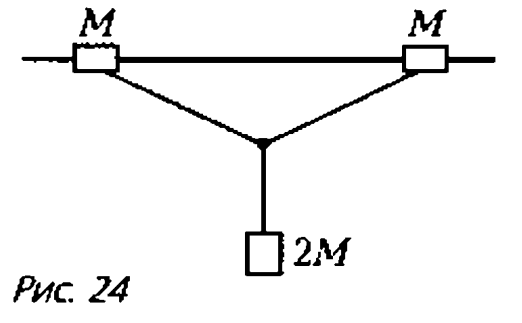
\includegraphics[scale=0.3]{images/1660.png}
		\end{center}

\textbf{1661.} გლუვ ჰორიზონტალურ მაგიდაზე იმყოფება სამი ერთნაირი ძელაკი. თითოეული მათგანის მასაა $M$. შუა ძელაკი მარცხენა კიდურა ძელაკთან შეერთებულია ძაფით, მარჯვენასთან კი $k$ სიხისტის მსუბუქი ზამბარით. თავდაპირველად სისტემას ისე აკავებენ, რომ ზამბარა არაა დეფორმირებული, ხოლო ძაფი არაა დაჭიმული, მაგრამ პრაქტიკულად არც ჩამოშვებულია. მარჯვენა ძელაკს ბიძგით მიანიჭეს მარჯვნივ მიმართული $v$ სიჩქარე. განსაზღვრეთ ძაფის რა სიგრძისთვის იქნება ძაფით შეერთებული ძელაკების შეჯახების ხმა ყველაზე ძლიერი. ძელაკები ყოველთვის წრფის გასწვრივ მოძრაობენ. ზამბარის დეფორმაციები ჰუკის კანონს ემორჩილება.
		\begin{center}
			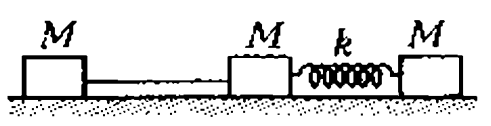
\includegraphics[scale=0.5]{images/F1661.png}
		\end{center}

\textbf{1669} ჰორიზონტალურ ზედაპირზე მოთავსებულია $M$ მასის გლუვი სოლი, ფუძესთან $\alpha$ კუთხით. ზედაპირზე ძევს აგრეთვე სოლის შემხები იგივე მასის კუბი (იხილე სურათი). კუბსა და ზედაპირს შორის ხახუნის კოეფიციენტია $\mu$. სოლზე მოათავსეს $m$ მასის ურიკა, რომელსაც სოლის ზედაპირზე ხახუნის გარეშე შეუძლია სრიალი და ხელი გაუშვეს. განსაზღვრეთ ურიკის შეძენილი სიჩქარე $h$ სიმაღლით დაწევისას (ამასთან ის ჯერ კიდევ სოლის ზედაპირზეა).
		\begin{center}
			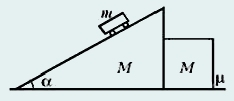
\includegraphics[scale=0.5]{images/F1669}
		\end{center}

\textbf{1671.} სამი პარალელური წვრილი არაგამტარი ღერო ჰორიზონტალურ სიბრტყეშია დამაგრებული. მეზობელ ღეროებს შორის მანძილია $d$. ღეროებზე წამოცმულია დამუხტული მძიმე შაიბები, რომელთაც ხახუნის გარეშე შეუძლიათ ღეროებზე სრიალი. თითოეული შაიბის მასაა $M$, ხოლო მუხტი $Q$. საწყის მომენტში სამი მათგანი ღეროების მართობ წრფეზე იმყოფებიან უძრავად, ხოლო მეოთხე მათგან შორსაა და მოძრაობს შუა ღეროზე $v_0$ სიჩქარით. განსაზღვრეთ შაიბების სიჩქარეები დიდი დროის შემდეგ. 
		\begin{center}
			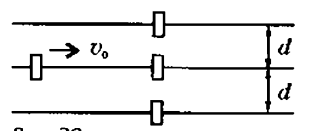
\includegraphics[scale=0.5]{images/F1671}
		\end{center}

\textbf{1674.} სურათზე გამოსახულ სისტემაში ჭოჭონაქების აჩქარებები ვერტიკალურადაა მიმართული, ძაფებიც ვერტიკალურია. განსაზღვრეთ რა ძალებით მოქმედებენ ჭოჭონაქებზე. ძაფების და ჭოჭონაქების მასები, აგრეთვე ხახუნი ჭოჭონაქების ღერძებთან უგულებელსაყოფად მცირეა. ძაფები უჭიმვადია.
		\begin{center}
			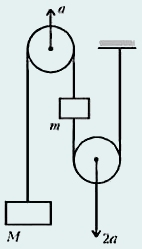
\includegraphics[scale=0.5]{images/F1674}
		\end{center}

\textbf{1676.} ჰაერში სხეულთა ვარდნის შესწავლისას მიიღეს საინტერესო შედეგები. ლითონის ბურთულა ვარდებოდა 100 მ/წმ დამყარებული სიჩქარით, ხოლო იგივე ლითონის  ორჯერ მეტი დიამეტრის მქონე ბურთულა ვარდებოდა 140 მ/წმ დამყარებული სიჩქარით. პატარა ბურთულას მიამაგრეს გრძელი ძაფი. ასეთი კუდით” ის ვარდებოდა 15 მ/წმ დამყარებული სიჩქარით. როდესაც “კუდი” ორჯერ დააგრძელეს, ვარდნის დამყარებული სიჩქარე 9 მ/წმ-მდე შემცირდა.  შეაფასეთ ამ ბურთულას ვარდნის  დამყარებული სიჩქარე ძალიან გრძელი “კუდის” შემთხვევაში. ჩათვალეთ, რომ “კუდი” მოძრაობისას ვერტიკალური რჩება. 

\textbf{1677.} ხისტ დახურულ ლიტრიან ჭურჭელში 900 გ წყალია. ჭურჭელში ჰაერი არ არის. ტემპერატურა ჭურჭლის შიგნით $+100 C$-ია. ჭურჭლის შიგთავსმა მიიღო 1000ჯ სითბოს რაოდენობა. შეაფასეთ ამ დროს აორთქლებული წყლის მასა. ჩათვალეთ, რომ ტემპერატურის $+101 C$-მდე აწევისას წყლის ნაჯერი ორთლის წნევა იზრდება 1 ატმ-დან 1.04 ატმ-მდე.

\textbf{1683.} ნაპირზე მყოფი ძრავა თანაბრად ახვევს ლილვზე თოკს, რომლის საშუალებით ნავს მიათრევენ ნაპირისკენ. დროის მოცემულ მომენტში თოკი ადგენს ჰორიზონტთან $\alpha$ კუთხეს, ნავის სიჩქარე კი $v$-ს ტოლია. თოკზე არის პატარა კვანძი, რომელიც ორჯერ უფრო ახლოა ნავთან, ვიდრე ლილვთან, რომელზეც თოკი ეხვევა. იპოვეთ ამ კვანძის სიჩქარე და აჩქარება დროის ამ მომენტში. 

\textbf{1689.} გლუვ ჰორიზონტალურ მაგიდაზე სრიალებს სწორი, ერთგვაროვანი $L$ სიგრძის ღერო. მოცემულ მომენტში ერთ-ერთი ბოლოს სიჩქარეა $v$ და ღეროსთან ადგენს $\alpha$ კუთხეს, ხოლო მეორე ბოლოს სიჩქარე ამ მომენტში $2v$-ს ტოლია. იპოვეთ მასათა ცენტრის სიჩქარე და ღეროს ბოლოების აჩქარებები ამ მომენტში. 

\textbf{1690.} დედამიწის ზედაპირიდან 1 კმ სიმაღლიდან დედამიწის ზედაპირის პარალელურად გაისროლეს პატარა სხეული. მისი სიჩქარე პირველ კოსმოსურ სიჩქარეზე 1$\%$-ით ნაკლებია. განსაზღვრეთ დედამიწის რომელ წერტილში დავარდება სხეული. დედამიწა მიიჩნიეთ იდეალურ ბირთვად, რომელზედაც არ არის ატმოსფერო. 

\textbf{1700.} საჭიროა იდეალური აირის გადაყვანა მდგომარეობიდან 1 ტემპერატურით $T_1$ მდგომარეობაში 2 ტემპერატურით $T_2>T_1$ ისე, რომ $1\rightarrow 2$ შებრუნებული პროცესის მიმდინარეობისას ტემპერატურა არ მცირდებოდეს და აირს არ ერთმეოდეს სითბო. ასეთი პროცესისას აირისათვის გადაცემული მინიმალური სითბოს რაოდენობაა $Q_1$. განსაზღვრეთ, პროცესის მიმდინარეობის მოცემულ პირობებში, რა მაქსიმალური სითბოს რაოდენობის გადაცემა შეიძლება აირისათვის.


\textbf{1704.} ჰორიზონტალური ღეროს გასწვრივ უხახუნოდ შეუძლია სრიალი $M$ მასის მძივის მარცვალს (იხილე სურათი). მარცვალზე მიბმულია $L$ სიგრძის მსუბუქი უჭიმვადი ძაფი. ძაფის თავისუფალ ბოლოს ისე ვეწევით, რომ მისი სიჩქარე ყოველთვის ძაფის გასწვრივაა მიმართული და მოდულით $v_0$-ია. განსაზღვრეთ ძაფის გამწევი ძალა იმ მომენტში, როდესაც ძაფი ღეროსთან $\alpha$ კუთხეს ადგენს.  ძაფი ყოველთვის ჰორიზონტალურ სიბრტყეშია.
		\begin{center}
			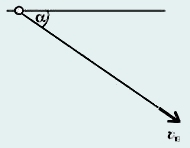
\includegraphics[scale=0.5]{images/F1704}
		\end{center}

\textbf{1705.} სურათზე გამოსახულ სისტემაში დიდ სხეულსა და ზედა ტვირთს შორის ხახუნის კოეფიციენტია $\mu_1$, ხოლო დიდ სხეულსა და ჰორიზონტალურ ზედაპირს შორის $\mu_2$. სხვაგან ხახუნი არ გვაქვს. განსაზღვრეთ რა პირობას უნდა აკმაყოფილებდეს ხახუნის კოეფიციენტები, რომ დიდი ტვირთი უძრავი იყოს.
		\begin{center}
			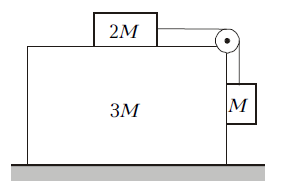
\includegraphics[scale=0.5]{images/F1705.png}
		\end{center}

\textbf{1707.} ვერტიკალური ცილინდრული ჭურჭელი შეიცავს ერთმანეთისაგან და გარემოსაგან ორი ერთნაირი მასიური დგუშით გამოყოფილ აირის ორ პორციას. თითოეული დგუშის მასაა $M$. ჭურჭლის ზედა ნაწილში ჟანგბადია, ხოლო ქვედაში - ჰელიუმი. თავდაპირველად აირების პორციების მოცულობა ერთნაირია და დგუშებს შორის მანძილია  $H$. ქვედა აირს ნელ-ნელა ათბობენ. განსაზღვრეთ სითბოს რა რაოდენობა უნდა გადავცეთ ჰელიუმს, რომ მისი მოცულობა ორჯერ გავზარდოთ? რისი ტოლი გახდება დგუშებს შორის მანძილი დიდი დროის შემდეგ, როდესაც აირების ტემპერატურები ხელახლა გატოლდება? ჭურჭლისა და დგუშების სითბოტევადობები უგულებელყავით. გარედან ჰაერი გამოტუმბულია. გარემოში სითბოს გაცემა უმნიშვნელოა. აირების პორციების გამყოფი დგუში ცუდი თბოგამტარია, ამიტომ ქვედა აირის გაცხელების დროში ზედა აირს სითბო პრაქტიკულად არ გადაეცემა.
		\begin{center}
			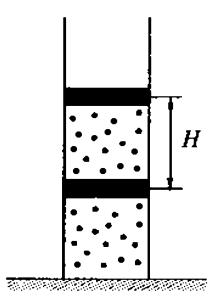
\includegraphics[scale=0.5]{images/F1707.png}
		\end{center}
	
\textbf{1718.} კურდღელი გარბოდა წრფის გასწვრივ 5 მ/წმ სიჩქარით. მას გაეკიდა მელია 4 მ/წმ სიჩქარით. ყოველ მომენტში მელიის სიჩქარე მიმართული იყო იმ წერტილისაკენ, სადაც მოცემულ მომენტში იმყოფებოდა კურდღელი. თავდაპირველად მათ შორის მანძილი მცირდებოდა, შემდეგ კი გაზრდა დაიწყო. მინიმალური მანძილი 30 მ აღმოჩნდა. განსაზღვრეთ მელიის აჩქარების მოდული იმ მომენტში, როდესაც მასსა და კურდღელს შორის მანძილი მინიმალური იყო.

\textbf{1719.} სურათზე გამოსახულ სისტემაში ხახუნი არ გვაქვს. $F$ ძალის რა მნიშვნელობისთვის შეუძლია სოლს და ურიკას ერთად, სრიალის გარეშე მოძრაობა ? დახრილი სიბრტყე ჰორიზონტისადმი დახრილია $\alpha$.
		\begin{center}
			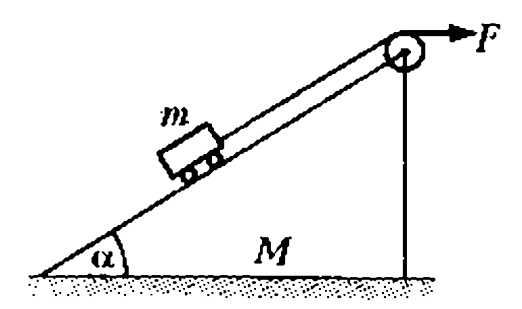
\includegraphics[scale=0.3]{images/1719.png}
		\end{center}

\textbf{1720.} ცარცის ნატეხი დევს ჰორიზონტალურ დაფაზე. მათ შორის ხახუნის კოეფიციენტია $\mu$. დაფამ უცებ დაიწყო მოძრაობა ჰორიზონტალური მიმართულებით $v_0$ სიჩქარით და $\tau$ დროის შემდეგ უცებ გაჩერდა. განსაზღვრეთ დაფაზე ცარცის მიერ დატოვებული კვალის სიგრძე.

\textbf{1728.} სინათლის წყარო თანაბრად მოძრაობს წრფის გასწვრივ $v=0.2c$ სიჩქარით, სადაც $c$ - სინათლის სიჩქარეა. დამკვირვებელი იმყოფება ამ წრფიდან $d$ მანძილით დაშორებულ წერტილში. დამკვირვებელთან მოსული სინათლის დაგვიანების გამო, მას წყაროს მოძრაობა არათანაბარი ეჩვენება. განსაზღვრეთ სინათლის წყაროს მაქსიმალური დაკვირვებული აჩქარება.   

\textbf{1730.} $S = 1\ \text{მ}^2$ ფუძის ფართობის მქონე ვერტიკალურ ცილინდრულ ჭურჭელში დგუში გაჩერებული ყავთ $h = 1\ \text{მ}$ სიმაღლეზე. ჭურჭელში $N = 100$ ცალი ერთნაირი $d = 0.1\ \text{მმ}$ დიამეტრის მქონე ბურთულებია. ისინი ქაოსურად მოძრაობენ. ბურთულას საშუალო კვადრატული სიჩქარეა $v_0 = 100\ \text{მ/წმ}$. დგუში აამოძრავეს $u = 1\ \text{მ/წმ}$ სიჩქარით და გააჩერეს $2h$ სიმაღლეზე. განსაზღვრეთ, რამდენჯერ შეიცვალა ბურთულას საშუალო ენერგია. დაჯახებებისას მექანიკური ენერგიის დანაკარგები არ გვაქვს. სიმძიმის ძალა არ მოქმედებს.

\textbf{1744.} კოსმოსის სიღრმეში დაფრინავს ძალიან დიდი ჭურჭელი, რომელშიც ქაოსურად მოძრაობენ ფოლადის პატარა ბურთულები. ბურთულების ნახევარს აქვს $d$ დიამეტრი, ხოლო ნახევარს - $2d$ დიამეტრი. ბურთულები დრეკადად ეჯახება ერთმანეთს და ჭურჭლის კედლებს, ენერგიის კარგვის გარეშე. რომელი დაჯახებებია უფრო ხშირი - მცირე ზომის ბურთულების ერთმანეთთან თუ დიდი ზომის ბურთულების ერთმანეთთან? რამდენჯერ?                      

\textbf{1745.} ძალიან დიდ ჭურჭელში იმყოფება $T_0=1000$ K ტემპერატურის და $p_0=0.1$ პა წნევის ჰელიუმი. $V=1$ ლ მოცულობის ჭურჭელი მოთავსებულია ამ დიდ ჭურჭელში. პატარა ჭურჭელში მაღალი ვაკუუმია. მცირე ჭურჭლის კედელში გახსნეს $S=1\ \text{მმ}^2$ ფართობის ხვრელი და $\tau=0.01$ წმ დროის შემდეგ დახურეს. შეაფასეთ წნევა და ტემპერატურა მცირე ჭურჭლის შიგნით მას შემდეგ, რაც მასში დამყარდება წონასწორობა. მცირე ჭურჭლის კედლები ძალზე თხელია, მაგრამ მათი თბოგამტარობა ძალზე მცირეა.  

\textbf{1752.} $M = 60\ \frac{\text{გ}}{\text{მოლი}}$ მოლური მასის აირი მოთავსებულია ხისტ კედლებიან ჰერმეტულ ჭურჭელში და უნარჩუნდება $T_0 = 0 \degree$ ტემპერატურა. მოლეკულების განივკვეთის ფართობია $S = 10^{-19}\ \text{მ}^2$. ისინი შეიძლება მივიჩნიოთ მყარ ბურთულებად. ექსპერიმენტის დასაწყისში აირის წნევაა $p_0 = 100$ პა. ულტრაიისფერი სინათლით აირის დასხივებისას მოლეკულები, რომლებიც შთანთქავენ სინათლის კვანტს, გადადიან აგზნებულ მდგომარეობაში. აგზნებულ მდგომარეობაში მოლეკულის სიცოცხლის საშუალო ხანგრძლივობაა $\tau = 10^{-3}$ წმ. ორი აგზნებული მოლეკულის დაჯახებისას მიმდინარეობს ქიმიური რეაქცია, რის შედეგადაც მიიღება ერთი ახალი მოლეკულა. ცნობილია, რომ ერთ წამში აირის ყოველ კუბურ სანტიმეტრში აღიგზნება $N = 10^{12}$ მოლეკულა. შეაფასეთ, რა დროში შემცირდება ჭურჭელში აირის წნევა თავდაპირველის $\epsilon = 1 \%$-ით.

\textbf{1757.} შუშისაგან დამზადებულ ფირფიტას კვეთაში აქვს ტოლფერდა ტრაპეციის ფორმა (იხ. ნახ.). ტრაპეციის ფუძეა $D$, სიმაღლე $L (D\ll L)$, ხოლო კუთხე ტრაპეციის გვერდებს შორის $\varphi \ll 1$–ს ტოლია. ფირფიტას გვერდითი წახნაგები მოვერცხლილია, შუშის გარდატეხის მაჩვენებელია $n$. სხივის დაცემის $\alpha$ კუთხის რა მნიშვნელობებისათვის ფირფიტას ფუძეზე დაცემული სხივი გაივლის ფირფიტაში?
		\begin{center}
			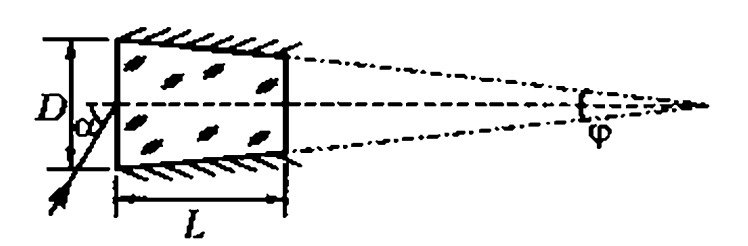
\includegraphics[scale=0.4]{images/F1757.png}
		\end{center}

\textbf{1758.} ???? კატა ლეოპოლდი ფარდულის სახურავის კიდეში იდგა. ორმა ბოროტმა წრუწუნამ მას შურდულიდან ესროლა. პირველი ქვა, რკალის შემოწერის წამის შემდეგ აირეკლა სახურავის დახრილი კიდიდან უშუალოდ კატის თათების მახლობლად და არეკვლიდან    წამის შემდეგ მოხვდა წრუწუნას თათებში (სურ. 20). განსაზღვრეთ წრუწუნასგან რა   მანძილითაა დაშორებული კატა ლეოპოლდი.                        

\textbf{1761.} მაღალ ვერტიკალურ ცილინდრულ ჭურჭელში, რომლის ფუძის ფართობია 10 $\text{სმ}^2$ და სიმაღლეა 1 მ, 2 კგ მასის დგუშის ქვეშ იმყოფება მშრალი ჰაერი და სამი პატარა ერთნაირი წყლიანი ამპულა. ატმოსფერული ჰაერის ტემპერატურაა $+100\ \degree C$, ატმოსფერული წნევა ნორმალურია. თავდაპირველად დგუში ჭურჭლის ფუძიდან 20 სმ სიმაღლეზეა გაჩერებული. მას შემდეგ რაც ერთ-ერთი ამპულა გასკდა, დგუში აიწია და საბოლოოდ 40 სმ სიმაღლეზე გაჩერდა. რამდენი წყალი იყო ამპულაში? ამოვარდება თუ არა დგუში ჭურჭლიდან თუ დანარჩენი ორი ამპულაც გასკდება?

\textbf{1762.} ორი არაგამტარი ნახევარსფეროს ცენტრები და მათი მაქსიმალური კვეთის სიბრტყეები ერთმანეთს ემთხვევა. მათი რადიუსებია $R$ და $r$, ხოლო მუხტები შესაბამისად $Q$ და $q$, მუხტი თანაბრადაა განაწილებული ნახევარსფეროების ზედაპირზე. განსაზღვრეთ მათი ურთიერთქმედების ძალა.
		\begin{center}
			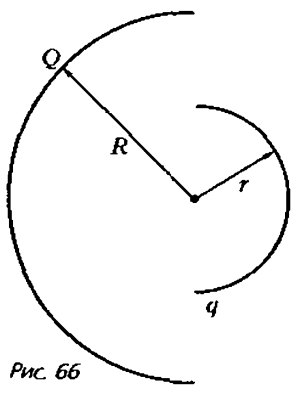
\includegraphics[scale=0.4]{images/F1762.png}
		\end{center}
	
\textbf{1763.} კომპიუტერულ სამყაროში ბგერის სიჩქარეა $c_1=3 \ \text{მ/წმ}$, ხოლო სინათლის სიჩქარე $c_2=8 \ \text{მ/წმ}$. პატარა ავტომობილი $v_0=5 \ \text{მ/წმ}$ სიჩქარით მოძრაობს სწორ გზაზე. დამკვირვებელი იმყოფება $L=20 \ \text{მ}$ დაშორებით ამ გზიდან. რა ადგილზე ხედავს დამკვირვებელი ავტომობილს, როცა მას ესმის მანქანის ხმა მათ შორის უმოკლესი მანძილიდან. (ჩათვალე რომ დამკვირვებელს ხმის საშუალებით ზუსტად შეუძლია ადგილმდებარეობის განსაზღვრა).

\textbf{1773.???} გაიშვიათებული ჰელიუმის მოლზე მიმდინარე პროცესი  $V-T$ დიაგრამაზე გამოისახება $V=V_0+\alpha T$ წრფის მონაკვეთით. აირის ტემპერატურა პროცესის განმავლობაში გაიზარდა $T_0$-დან $3T_0$-მდე  ($V_0$, $T_0$ და $\alpha$ მუდმივები ცნობილად ითვლება). განსაზღვრეთ ამ პროცესის დროს აირის მაქსიმალური და მინიმალური სითბოტევადობები.

\textbf{1854.} პიტერი და პაული დარბიან ფეხბურთის მინდორზე (ეტყობა, სადღაც ბავარიაში), ამასთან მათ შორის მანძილი მუდმივად 50 მ-ია. პიტერი მოდულით 2 მ/წმ სიჩქარით დარბის 50 მ რადიუსის წრეწირზე, ხოლო პაული დარბის ამ წრეწირის ცენტრზე გამავალი წრფის გასწვრივ. განსაზღვრეთ პაულის მაქსიმალური სიჩქარე და აჩქარება. მიიჩნიეთ, რომ ერთ ადგილზე ის დიდხანს არ დგას.

\textbf{1855.} სურათზე გამოსახულ სისტემაში ყველა ჭოჭონაქი უწონოა, ხოლო ძაფები უწონო და უჭიმვადია. ყველა ძაფის ჭოჭონაქზე გადაუდებელი ნაწილები ვერტიკალურია. სხეულების მასები ერთნაირია. განსაზღვრეთ ჭოჭონაქების აჩქარებები. 
		\begin{center}
			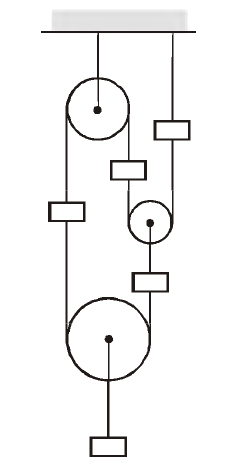
\includegraphics[scale=0.5]{images/F1855.png}
		\end{center}
	
\textbf{1998.} ავტომობილი მოძრაობს სწორ გზაზე. მოძრაობის პირველ საათში მისი საშუალო სიჩქარე შეადგენდა 50 კმ/სთ, კიდევ ერთი საათი იმოძრავა 70 კმ/სთ საშუალო სიჩქარით. შემდგომი ერთი საათი იდგა საცობში. ხოლო დარჩენილი გზა გაიარა მუდმივი 40 კმ/სთ სიჩქარით. განსაზღვრეთ ავტომობილის საშუალო სიჩქარე მოძრაობის მთელ გზაზე.

\textbf{2024.} ჩვეულებრივ ცვლადი დენის ქსელში 220 ვ, 50 ჰც ჩართულია მიმდევრობით შეერთებული 1 მკფ ტევადობის კონდენსატორი და გამახურებელი-რეზისტორი. განსაზღვრეთ  ასეთი გამაცხელებლის მაქსიმალური სიმძლავრე. რატომ დაგვჭირდა კონდენსატორის ჩართვა ? 
სურათია საჭირო. (an ki an ara)

\textbf{2154.} გლუვ ჰორიზონტალურ ზედაპირზე უძრავად დევს მონეტა, რომლისკენაც მოსრიალებს ისეთივე მონეტა. აბსოლიტურად დრეკადი დაჯახების შემდეგ მონეტების სიჩქარე აღმოჩნდა მოდულით ტოლი. განსაზღვრეთ გაფანტვის კუთხე.

\textbf{2235.} სწორ გზაზე მუდმივი $v$ სიჩქარით მოძრაობს ავტომობილი. დროის რაღაც მომენტში ავტომობილი უძრავ დამკვირვებელს უახლოვდებოდა $u\ (u<v)$. ამ მომენტიდან $t$ დროის შემდეგ ავტომობილი აღმოჩნდა დამკვირვებლიდან უახლოეს მანძილზე. გზიდან რა $L$ მანძილზე იმყოფება დამკვირვებელი ? 

\textbf{2420.} გზის პირველი ნახევარი ავტობუსმა გაიარა 8-ჯერ მეტი სიჩქარით ვიდრე მეორე ნახევარი. ავტობუსის საშუალო სიჩქარე მოძრაობის სრულ გზაზე ტოლია 16 კმ/სთ. იპოვეთ ავტობუსის საშუალო სიჩქარე მოძრაობის დროის პირველ მესამედში.

\textbf{2422.} ოთხი ერთნაირი $L$ სიგრძის ყინულის აგური დაალაგეს ისე როგორც ნახაზზეა ნაჩვენები. რა მაქსიმალური $x$ მანძილით შეიძლება გავწიოთ მარჯვენა აგური, რომლისთვისაც აგურების სისტემა არ დაინგრევა. ჩათვალე რომ აგურები გლუვია და სიმძიმის ძალა მოდებულია აგურის გეომეტრიულ ცენტრში.
		\begin{center}
			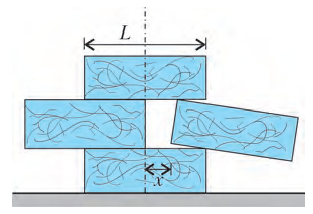
\includegraphics[scale=0.6]{images/F2422.png}
		\end{center}

\textbf{2531.} "ნაცრისფერ" ყუთში მოთავსებულია 6 მიმდევრობით შეერთებული წინაღობისაგან შემდგარი რგოლი. (იხილე ნახაზი). ყუთში არსებული სპეციალური ხუფის საშუალებით შესაძლებელია გავხსნათ მხოლოდ ერთი რეზისტორის გამომყვანი კონტაქტები და ომმეტრის საშუალებით გავზომოთ ამ ორ წერტილს შორის წინაღობა. ექსპერიმენტის განმავლობაში მიიღეს 6 მნიშვნელობა. $R_{12}$, $R_{23}$, $R_{34}$, $R_{45}$, $R_{56}$, $R_{61}$. (მეორე ინდექსი აღნიშნავს წინაღობის ნომერს). ამ მონაცემებით განსაზღვრეთ ექვსივე წინაღობის მნიშვნელობა.
	\begin{center}
		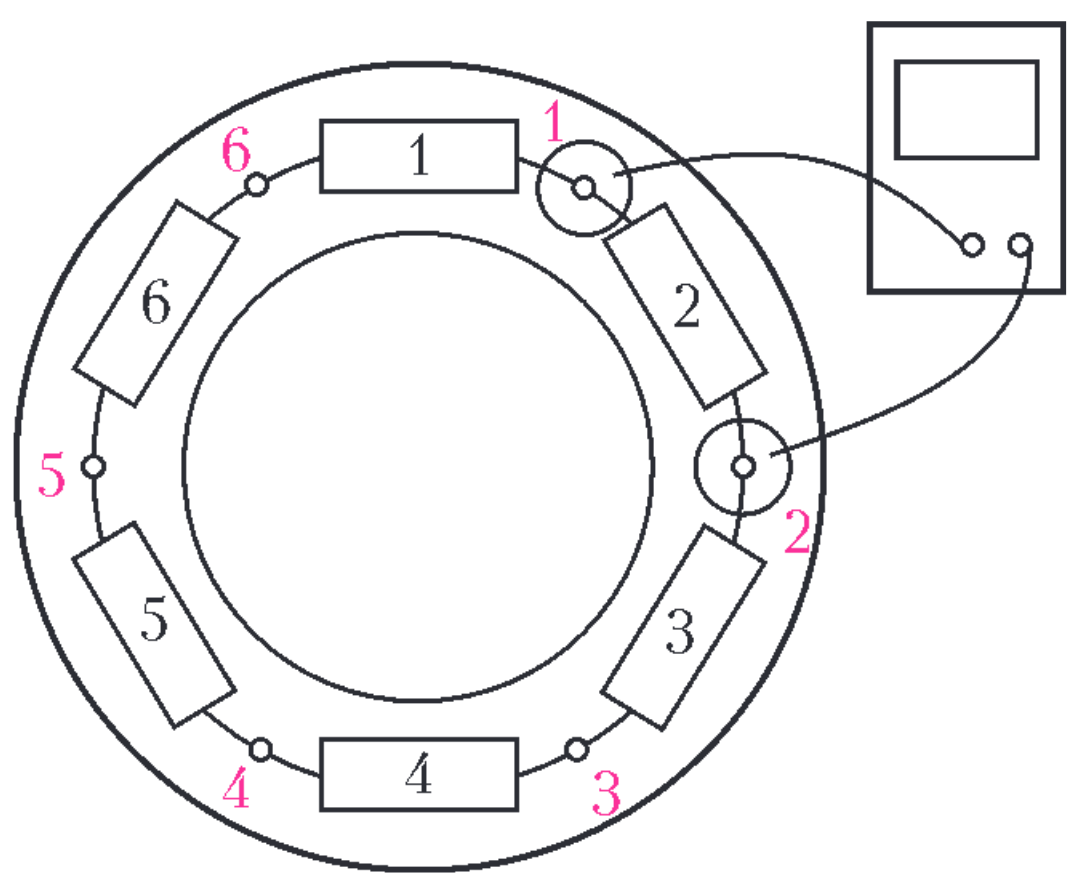
\includegraphics[scale=0.3]{images/F2531.png}
	\end{center}

\textbf{2604.} 

\textbf{????.} $m$ მასის ერთგვაროვანი ფიცარი დევს ურთიერთსაწინააღმდეგო მიმართულებებით დიდი სისწრაფით მბრუნავ ორ ლილვზე იხილე ნახაზი. ლილვების ცენტრებს შორის მანძილია $l$, ლილვებსა და ფიცარს შორის სრიალის ხახუნის კოეფიციენტია $\mu$. განსაზღვრეთ ფიცრის გრძივი რხევების სიხშირე.
	ნახატი უნდა დაემატოს\\
	
\textbf{????.} სინათლის წერტილოვანი წყარო მოძრაობს მუდმივი V სიჩქარით წრფეზე, რომელიც შეადგენს შემკრები ლინზის მთავარ ოპტიკურ ღერძთან  პატარა $\alpha$ კუთხეს. წყაროს ტრაექტორია გადაკვეთს მთავარ ოპტიკურ რერძს ლინზიდან ორმაგ ფოკუსურ მანძილზე. რისი ტოლია ლინზაში მიღებული გამოსახულების სიჩქარის მინიმალური მნიშვნელობა თვით მოძრავი წყაროს მიმართ?

\textbf{????.} თხელი ლინზის საშუალებით A წერტილში მიიღება წერტილოვანი სინათლის წყაროს ნამდვილი გამოსახულება. როდესაც ეს ლინზა შეცვალეს ამავე წერტილში განლაგებული სხვა ლინზით, გამოსახულებამ გადაინაცვლა B წერტილში (იხ. ნახ.). შემდეგ პირველი ლინზა მჭიდროდ მიადგეს მეორეს და ამ შემთხვევაში იმავე წყაროს გამოსახულება მიიღებოდა ჩ წერტილში. აგებით დაადგინეთ წერტილოვანი წყაროს ადგილმდებარეობა.

\textbf{????.} ნახატზე მოყვანილია შემკრები ლინზის მთავარი ოპტიკური რერძი, მისი ფოკუსების განლაგება, თვით ლინზის ზომები და ასევე სინათლის წერტილოვანი წყარო. მიუთითეთ ერთი წერტილი მაინც, საიდანაც არ ჩანს არც სინათლის წყარო და არც მისი გამოსახულება ლინზაში. ასევე მიუთითეთ ის წერტილი, საიდანაც ერთდროულად ჩანს სინათლის წყაროც და მისი გამოსახულებაც.

\textbf{????.} ბრტყელ-ჩაზნექილი ლინზის ბრტყელი ზედაპირი მოვერცხლილია. ლინზის ფოკუსური მანძილია $F$. ლინზიდან $d$ მანძილზე მთავარ ოპტიკურ ღერძზე განლაგებულია წერტილოვანი წყარო. სად არის მისი გამოსახულება ? 

\textbf{????.} ვერტიკალურ ცილინდრულ ჭურჭელში, რომლის ფართობია 1 მ2, 1მ სიმაღლეზე განლაგებულია დგუში. დგუში ქვეშ ცილინდრშია 100 ერთნაირი ბურთულა. ბურთულების დიამეტრი 0.1მმ. ბურთულები მოძრაობენ ქაოტურად ისე, რომ მათი საშუალო კვადრატული სიჩქარეა 100 მ/წმ. დგუში მოძრაობს გარეშე ძალის მოქმედებით და 2 მ სიმაღლეზე აჩერებენ. რამდენჯერ შეიცვლება ამის შედეგად ბურთულების საშუალო ენერგია ? დაჯახებებია აბსოლუტურად დრეკადია, სიმძიმის ძალა არ მოქმედებს. 

\textbf{1643.} ჰორიზონტალურ საყრდენზე იმყოფება მსუბუქი უჭიმვადი ძაფით შეერთებული ორი ერთნაირი დიდი ძელაკი (სურ. 11). თითოეული მათგანის მასაა  . ძელაკებსა და საყრდენს შორის ხახუნის კოეფიციენტია  . ძაფი არაა მოშვებული. პირველი ძელაკის ზედა გლუვ ზედაპირზე იმყოფება პატარა   მასის ტვირთი. საყრდენს ამოძრავებენ ჰორიზონტალური მიმართულებით ძაფის პარალელურად პირველი ძელაკის მხარეს დიდი სიჩქარით. იპოვეთ ძაფის დაჭიმულობის ძალა ძელაკიდან ტვირთის ჩამოვარდნამდე.

\textbf{1645.} დედამიწის ჰორიზონტალური ზედაპირიდან დიდ   სიმაღლეზე დამაგრებულ მსუბუქ ჭოჭონაქზე გადადებულია მოქნილი თოკი (სურ. 12). თოკის ბოლოები მიწაზე ქმნიან გროვებს, რომლებიც ხელს არ უშლიან თოკის მოძრაობას. ერთ მხარეს თოკს მოეჭიდა   მასის ადამიანი, რომელიც  ხელების სწრაფი მორიგეობითი  გადატანით ითრევს თოკს ისე, რომ ცდილობს დედამიწის ზედაპირიდან ერთ სიმაღლეზე რჩებოდეს. თოკის განსაზღვრული დამყარებული სიჩქარით მოძრაობისას, მან ეს მოახერხა. განსაზღვრეთ ეს სიჩქარე. თოკის ერთეული სიგრძის მასაა  , თავისუფალი ვარდნის აჩქარებაა  . ხახუნი ჭოჭონაქში არ გვაქვს.                                                                                                             

\textbf{1749.} გლუვ ჰორიზონტალურ მაგიდაზე მოთავსებულია   სიგრძის ჰანტელი. ის წარმოადგენს უწონო ხისტი ერთგვაროვანი ღეროთი შეერთებულ ორ ერთნაირ პატარა ბურთულას (სურ. 19). თითოეული ბურთულას მასაა  . გარკვეულ მომენტში ჰანტელზე მოქმედება დაიწყო ჰორიზონტალურ სიბრტყეში ურთიერთსაწინააღმდეგოდ მიმართულმა ორმა ძალამ. ორივე ძალა ჰანტელის ღეროს მართობულია. თითოეული მათგანის მოდულია  . ერთი ძალა მოდებულია ღეროს ცენტრში, მეორე კი ერთ-ერთ ბურთულაზე. ძალები მუდმივად რჩება ღეროს მართობული და ნახსენებ წერტილებში მოდებული. როგორ იმოძრავებს ღერო? რა დროში მობრუნდება ის   კუთხით? რისი ტოლი იქნება ამ მომენტში ღეროს დაჭიმულობის ძალა?                                              

\textbf{1834.} უწონო ზამბარების ერთ ბოლოებთან  მიმაგრებულია სხეულები, ხოლო მეორე ბოლოები მიმაგრებულია კედლებთან (სურ. ). სხეულები ძაფების მეშვეობით გაჩერებულია კედლებიდან   მანძილზე. არადეფორმირებული ზამბარების სიგრძეებია  . კედლებს შორის მანძილია  . ძაფები ერთდროულად გადაწვეს. ამის შემდეგ სხეულები მიეჯახნენ ერთმანეთს და მიეწებნენ. განსაზღვრეთ დაჯახების შემდეგ რხევებისას სხეულების მაქსიმალური სიჩქარე. დაჯახება ცენტრულია. ზამბარების სიხისტეები და სხეულების მასები მითითებულია სურათზე. ხახუნი და სხეულების ზომები უგულებელყავით.


თერმოდინამიკა

\textbf{1595.} ვერტიკალურ ჭურჭელში მძიმე დგუშის ქვეშ იმყოფება ჰელიუმის მცირე რაოდენობა. ატმოსფერული წნევა არ გვაქვს. დგუში გაჩერებულია ჭურჭლის ფუძიდან   სიმაღლეზე. დგუში ძალიან სწრაფად ასწიეს ჭურჭლის ფსკერიდან   სიმაღლეზე და გაათავისუფლეს. განსაზღვრეთ რა სიმაღლეზე გაჩერდება დგუში რხევების მილევის შემდეგ. ჭურჭელი თბოგაუმტარია. ჭურჭლის და დგუშის სითბოტევადობა შეიძლება უგულებელყოთ. ხახუნი დგუშსა და ჭურჭლის კედლებს შორის მცირეა. რამდენიმე ზედმეტი მონაცემი ამ ამოცანისათვის: დგუშის მასა  , თავისუფალი ვარდნის აჩქარება  , ჭურჭლის ფსკერის შიგა ფართობი  . რა უნდა გვესმოდეს გამოთქმაში “ძალიან სჭრაფად ასწიეს”? როგორ შეიცვლება პასუხი. თუ დგუშს ძალიან ნელა ავწევთ?


\textbf{1662.} ვერტიკალურ თბოიზოლირებულ ცილინდრულ ჭურჭელში მძიმე დგუშის ქვევით აზოტია. დგუშზე ზემოდან დაყრილია ქვიშის გროვა. სისტემა წონასწორობაშია. საწყისი მოცულობაა  , ხოლო წნევა  . დაიწყეს ქვიშის მარცვალ-მარცვალ ნელი მოშორება დგუშიდან მანამ, სანამ წნევა არ შემცირდა  -მდე. ამ დროს აირის მოცულობა გაიზარდა  -მდე (რა თქმა უნდა ამ მოცულობის გამოთვლა შეიძლებოდა, მაგრამ ჩავთვალოთ, რომ ეს უკვე გააკეთეს და თქვენ გითხრეს შედეგი). ახლა ექსპერიმენტი განსხვავებულად ჩავატაროთ მთელი ქვიშის გროვა ერთბაშად ავიღოთ დგუშიდან. განსაზღვრეთ, რა კინეტიკური ენერგია ექნებოდა დგუშს იმ მომენტში, როდესაც აირის მოცულობა  -ის ტოლი იქნებოდა. აირი საკმარისადაა გაუხშოებული.

\textbf{1670.} ფართობის და   სიმაღლის ოთახში ჰაერი ნორმალურ პირობებშია. შეაფასეთ რამდენი მოლეკულა ეჯახება ჭერს  -ის განმავლობაში. ოთახის ჭერს თუ იატაკს ეჯახებიან მოლეკულები უფრო ხშირად? შეაფასეთ   დროში იატაკთან და ჭერთან მოლეკულების დაჯახებათა რიცხვის სხვაობა. ოთახში ტემპერატურა ყველგან ერთნაირად მიიჩნიეთ.

\textbf{1692.} პლანეტის ზედაპირი, რომლის ზომები, მასა და ატმოსფეროს შემადგენლობა ისეთივეა, როგორც დედამიწის, სრულად იყო დაფარული ყველგან ერთნაირი  230 მ სიღრმის და   ტემპერატურის ოკეანით. შინაგანი პროცესების შედეგად ტემპერატურამ ყველგან  -მდე აიწია, მაგრამ ოკეანის სიღრმე არ შეიცვალა. ჩათვალეთ, რომ პლანეტის მყარი ნაწილის ზომები გათბობისას არ შეცვლილა და განსაზღვრეთ წყლის მოცულობითი გაფართოების საშუალო კოეფიციენტი აღნიშნულ ტემპერატურულ დიაპაზონში.

\textbf{1722.} დახშულ ჭურჭელში ჰაერთან ერთად იმყოფება წყლის გარკვეული რაოდენობა. ჭურჭლის შიგნით ნარჩუნდება   ტემპერატურა. ჭურჭლის თავდაპირველი მოცულობაა 10 ლ, სითხეს ამ დროს ჭურჭლის მცირე ნაწილი უკავია, ხოლო წნევა 2 ატმოსფეროა. როდესაც ჭურჭლის მოცულობა 20 ლ=მდე გაზარდეს, ჭურჭელში აირის წნევა 1.4 ატმოსფერომდე დაეცა. განსაზღვრეთ ჭურჭელში მყოფი ჰაერის მასა. წყლის რამდენი მოლეკულაა ჭურჭელში?

\textbf{1723.} მაღალ ვერტიკალურ ჭურჭელში   მასის დგუშის ქვეშ იმყოფება მცირე რაოდენობის ჰელიუმი. დგუშს ადევს    მასის საწონი. წონასწორობის მდგომარეობაში დგუში ფსკერიდან   სიმაღლეზეა. საწონი აიღეს დგუშიდან და მან დაიწყო ზევით მოძრაობა. შეაფასეთ დგუშის აწევის მაქსიმალური სიმაღლე. ფსკერიდან რა სიმაღლეზე გაჩერდება საბოლოოდ დგუში? გამოთვლებისას ჩათვალეთ, რომ ხახუნი მცირეა, ჭურჭლის კედლები და დგუში თბოგაუმტარია, ხოლო ჭურჭლის და დგუშის სითბოტევადობები ძალზე მცირეა.

\chapter{თემატური საძიებელი}

$\ \quad$ კინემატიკა: 44; 754; 1283; 1418; 1763; 1854; 1998; 2235; 2420;

დინამიკა: 1719; 

ენერგია: 1660;

სტატიკა: 724; 1124; 1508; 2422

სითბური გაფართოება: 338;

წრედები: 1006; 1320;

ცვლადი დენი: 2024

სითბო: 649; 1065; 1215; 1633; 1737; 1744; 

ოპტიკა: 1332; 1347;
\chapter{პასუხები}

\textbf{32.} მეორე მდგომარეობა. \\
\textbf{37.} $\rho glS_1S_2/(S_1-S_2)$. \\
\textbf{63.} ადამიანი შეიანარჩუნებს წონასწორობას, თუკი გორაკიდან მოქმედი რეაქციის ძალა გადის მის მასათა ცენტრში. \\ 
\textbf{97.} ნავში (თუ მისი კედლები სქელია). \\
\textbf{179}: $v(\tau_0-\tau)/(\tau_0+\tau)$. \\
\textbf{188.} $P\tau+(ct+\lambda)\rho n$. \\
\textbf{297.} $\pi p(R^2-r^2)$. \\
\textbf{723.} $l_0(u-v)/(u+v)$. \\
\textbf{724.} $5F/k$. \\
\textbf{844.} $(m-\rho_0 V)/(\alpha V)$ ორივე შემთხვევაში.\\
\textbf{1006.} 8/3 ომი. \\
\textbf{1065.} 42 წმ. \\
\textbf{1320.} $R_x=20$ ომი, $R_y=10$ ომი.\\
\textbf{1332.} 4 სმ, 12 სმ. \\
\textbf{1347.} 10.5 სმ და 18.5 სმ. \\
\textbf{1388.} $2m\alpha v_0^2$. \\
\textbf{1418.} $vr/R$. \\
\textbf{1508.} $2\pi\mu T$. \\
\textbf{1609.} $\dfrac{v^2}{4\mu g}$. \\
\textbf{1633.} $1-\dfrac{T_2}{T_1}$. \\
\textbf{1660.} $\sqrt{2gL}$ და $2\sqrt{\dfrac{gL}{3\sqrt{3}}}$. \\
\textbf{1718.} 0.4 $\text{მ}/\text{წმ}^2$. \\
\textbf{1719.} $\dfrac{mg\sin\alpha}{1-\dfrac{m\cos\alpha}{M+m}}$. \\
\textbf{1720.} \\
\textbf{1730.} ენერგია შემცირდა 4/3 ჯერ. დიდი დროის შემდეგ საშუალო კვადრატული სიჩქარე გახდება $v_0 \sqrt{3/4} = 87\ \text{მ/წმ}$ \\
\textbf{1744.} დიდი ბურთელები ეჯახებიან ერთმანეთს $\sqrt{2}$-ჯერ უფრო ხშირად. \\
\textbf{1763.} უახლოესი წერტილიდან $\approx 17$ მეტრის მოშორებით. \\
\textbf{1854.} 4 მ/წმ და 0.16 $\text{მ}/\text{წმ}^2$. \\
\textbf{1998.} 40 კმ/სთ. \\
\textbf{2154.} $90 \degree$. \\
\textbf{2235.} $L=\dfrac{vt\sqrt{v^2-u^2}}{u}$; \\
\textbf{2420.} 30 კმ/სთ. \\
\textbf{2422.} $x\approx0.21L$. \\
\textbf{2531.} 
\end{document}
